\documentclass[british]{scrreprt}

\usepackage{scrhack}
\usepackage{amsmath}
\usepackage{amssymb}
\usepackage{pifont}
\usepackage{fontspec}
\usepackage[math-style = ISO, bold-style = ISO]{unicode-math}
\usepackage{mathtools}
\usepackage{xfrac}
\usepackage[verbose = silent]{microtype}
\usepackage[urldate = iso, seconds = true, sortcites = true]{biblatex}
\usepackage[useregional]{datetime2}
\usepackage{minted}
\usepackage{csquotes}
\usepackage{epigraph}
\usepackage{graphicx}
\usepackage{pdfpages}
\usepackage{booktabs}
\usepackage{longtable}
\usepackage{siunitx}
\usepackage{threeparttable}
\usepackage{tabu}
\usepackage[hidelinks]{hyperref}
\usepackage{subcaption}
\usepackage{enumitem}
\usepackage{calc}
\usepackage{physics}
\usepackage[xindy, toc, numberedsection]{glossaries}
\usepackage{algorithm2e}
\usepackage{tikz}
\usepackage{pgfplots}
\usepackage{xcolor}
\usepackage[standard, amsmath, hyperref]{ntheorem}
\usepackage[nameinlink]{cleveref}
\usepackage{pdflscape}
\DeclareDocumentCommand{\todo}{m}{}
%\usepackage{luatodonotes}
\usetikzlibrary{shapes.geometric}

\KOMAoptions{
	abstract = true,
	chapterprefix = true,
}
\setkomafont{disposition}{\normalcolor\bfseries}
\renewcommand*{\chapterformat}{%
\mbox{\chapappifchapterprefix{\nobreakspace}\thechapter\IfUsePrefixLine{}{\enskip}}
}
\renewcommand{\chapterlineswithprefixformat}[3]{%
	\centering
	{\normalfont\textsc{#2}}\hrule\par\bigskip#3\par\bigskip\hrule%
}

\setmainfont{TeX Gyre Pagella}
\setsansfont{Open Sans}
\setmonofont{Fira Code}
\setmathfont{TeX Gyre Pagella Math}

\renewcommand{\mkbegdispquote}[2]{\itshape}
\renewcommand{\mkenddispquote}[2]{#1\\\normalfont#2}
\renewcommand{\mkcitation}[1]{\textemdash~#1}

% https://tex.stackexchange.com/a/537722/105667
\newrobustcmd*{\citefullauthor}{\AtNextCite{\DeclareNameAlias{labelname}{given-family}}\citeauthor}

\crefname{Definition}{definition}{definitions}

\setminted{
	autogobble = true,
	breaklines = true,
	tabsize = 2,
    linenos = true
}
\setminted[xml]{
    breakbefore = <,
    breakafter  = >
}
\setminted[R]{
    breakafter = {:},
    breakaftergroup = true
}

\sisetup{
	table-text-alignment = left,
	table-number-alignment = right,
}

\renewcommand{\laplacian}{\increment}
\newcommand{\R}{\mathbb{R}}
\DeclareMathOperator{\prob}{\mathbb{P}}
\DeclareMathOperator{\cov}{cov}
\DeclareMathOperator{\cor}{cor}
\DeclareMathOperator{\BesselK}{K}
\newcommand{\graphprod}{\mathbin{\square}}
\newcommand{\adj}{\mathbin{\sim}}

\makeglossaries
\renewcommand{\glsnamefont}{\normalfont\bfseries}
%\setacronymstyle{long-sc-short}
\newacronym{hpc}{HPC}{high-performance computing}
\newacronym[description = {Swiss Federal Institute of Technology}]{eth}{ETH}{Eidgenössiche Technische Hochschule}
\newacronym{pde}{PDE}{partial differential equation}
\newacronym{spde}{SPDE}{stochastic \acrshort{pde}}
\newacronym{gf}{GF}{Gaussian field}
\newacronym{grf}{GRF}{Gaussian \acrlong{rf}}
\newacronym{rf}{RF}{random field}
\newacronym{mrf}{MRF}{Markov \acrlong{rf}}
\newacronym{gmrf}{GMRF}{Gaussian \acrlong{mrf}}
\newacronym{inla}{INLA}{integrated nested Laplacian approximation}
\newacronym{usi}{USI}{Università della Svizzera italiana}
\newacronym{cad}{CAD}{computer-aided design}
\newacronym{cli}{CLI}{command-line interface}
\newacronym{api}{API}{application programming interface}
\newacronym{xml}{XML}{extensible markup language}
\newacronym{xdmf}{XDMF}{extensible data model and format}
\newacronym{hdf}{HDF}{hierarchical data format}
\newacronym{hdf5}{HDF5}{\acrlong{hdf}, version 5}
\newacronym{fem}{FEM}{finite element method}
\newacronym{demf}{DEMF}{diffusion-based extension of the Gaussian Matérn field}
\newacronym{mcmc}{MCMC}{Markov chain Monte Carlo method}
\newacronym{spd}{spd}{symmetric positive-definite}

\definecolor{ETH1}{cmyk/RGB/HTML}{1.00, 0.70, 0.00, 0.30 /  31,  64, 122 / 1F407A} % dark blue
\definecolor{ETH2}{cmyk/RGB/HTML}{0.75, 0.40, 1.00, 0.40 /  72,  90,  44 / 485A2C} % dark green
\definecolor{ETH3}{cmyk/RGB/HTML}{1.00, 0.50, 0.00, 0.00 /  18, 105, 176 / 1269B0} % blue
\definecolor{ETH4}{cmyk/RGB/HTML}{0.30, 0.00, 1.00, 0.55 / 114, 121,  28 / 72791C} % green
\definecolor{ETH5}{cmyk/RGB/HTML}{0.20, 1.00, 0.00, 0.20 / 145,   5, 106 / 91056A} % magenta
\definecolor{ETH6}{cmyk/RGB/HTML}{0.00, 0.00, 0.00, 0.70 / 111, 111, 111 / 6F6F6F} % gray
\definecolor{ETH7}{cmyk/RGB/HTML}{0.00, 0.90, 0.80, 0.20 / 168,  50,  45 / A8322D} % red
\definecolor{ETH8}{cmyk/RGB/HTML}{1.00, 0.25, 0.30, 0.10 /   0, 122, 150 / 007A96} % cyan
\definecolor{ETH9}{cmyk/RGB/HTML}{0.00, 0.55, 1.00, 0.40 / 149,  96,  19 / 956013} % brown

\colorlet{ETHDarkBlue}{ETH1}
\colorlet{ETHDarkGreen}{ETH2}
\colorlet{ETHBlue}{ETH3}
\colorlet{ETHGreen}{ETH4}
\colorlet{ETHMagenta}{ETH5}
\colorlet{ETHGray}{ETH6}
\colorlet{ETHRed}{ETH7}
\colorlet{ETHCyan}{ETH8}
\colorlet{ETHBrown}{ETH9}

\definecolor{ETH180}{cmyk/RGB/HTML}{0.80, 0.52, 0.00, 0.24 /  56,  92, 155 / 385C9B}
\definecolor{ETH160}{cmyk/RGB/HTML}{0.60, 0.39, 0.00, 0.18 / 116, 141, 185 / 748DB9}
\definecolor{ETH140}{cmyk/RGB/HTML}{0.40, 0.22, 0.00, 0.12 / 160, 177, 208 / A0B1D0}
\definecolor{ETH120}{cmyk/RGB/HTML}{0.20, 0.10, 0.00, 0.06 / 205, 214, 230 / CDD6E6}
\definecolor{ETH110}{cmyk/RGB/HTML}{0.10, 0.05, 0.00, 0.05 / 230, 235, 243 / E6EBF3}

\definecolor{ETH280}{cmyk/RGB/HTML}{0.52, 0.05, 0.80, 0.53 / 103, 128,  78 / 67804E}
\definecolor{ETH260}{cmyk/RGB/HTML}{0.39, 0.00, 0.60, 0.42 / 141, 160, 122 / 8DA07A}
\definecolor{ETH240}{cmyk/RGB/HTML}{0.26, 0.00, 0.40, 0.28 / 179, 192, 167 / B3C0A7}
\definecolor{ETH220}{cmyk/RGB/HTML}{0.13, 0.00, 0.20, 0.14 / 217, 223, 211 / D9DFD3}
\definecolor{ETH210}{cmyk/RGB/HTML}{0.07, 0.00, 0.10, 0.07 / 236, 239, 233 / ECEFE9}

\definecolor{ETH380}{cmyk/RGB/HTML}{0.80, 0.40, 0.00, 0.00 /  65, 135, 192 / 4187C0}
\definecolor{ETH360}{cmyk/RGB/HTML}{0.60, 0.30, 0.00, 0.00 / 113, 165, 208 / 71A5D0}
\definecolor{ETH340}{cmyk/RGB/HTML}{0.40, 0.20, 0.00, 0.00 / 160, 195, 223 / A0C3DF}
\definecolor{ETH320}{cmyk/RGB/HTML}{0.20, 0.10, 0.00, 0.00 / 208, 225, 239 / D0E1EF}
\definecolor{ETH310}{cmyk/RGB/HTML}{0.10, 0.05, 0.00, 0.00 / 231, 240, 247 / E7F0F7}

\definecolor{ETH480}{cmyk/RGB/HTML}{0.24, 0.00, 0.80, 0.44 / 142, 148,  73 / 8E9449}
\definecolor{ETH460}{cmyk/RGB/HTML}{0.18, 0.00, 0.60, 0.33 / 170, 175, 119 / AAAF77}
\definecolor{ETH440}{cmyk/RGB/HTML}{0.12, 0.00, 0.40, 0.22 / 199, 201, 164 / C7C9A4}
\definecolor{ETH420}{cmyk/RGB/HTML}{0.06, 0.00, 0.20, 0.11 / 227, 228, 210 / E3E4D2}
\definecolor{ETH410}{cmyk/RGB/HTML}{0.04, 0.00, 0.10, 0.06 / 241, 241, 232 / F1F1E8}

\definecolor{ETH580}{cmyk/RGB/HTML}{0.16, 0.80, 0.00, 0.16 / 167,  55, 136 / A73788}
\definecolor{ETH560}{cmyk/RGB/HTML}{0.12, 0.60, 0.00, 0.12 / 189, 105, 165 / BD69A5}
\definecolor{ETH540}{cmyk/RGB/HTML}{0.08, 0.40, 0.00, 0.08 / 211, 155, 195 / D39BC3}
\definecolor{ETH520}{cmyk/RGB/HTML}{0.05, 0.20, 0.00, 0.04 / 233, 205, 225 / E9CDE1}
\definecolor{ETH510}{cmyk/RGB/HTML}{0.04, 0.12, 0.00, 0.00 / 244, 230, 240 / F4E6F0}

\definecolor{ETH680}{cmyk/RGB/HTML}{0.00, 0.00, 0.00, 0.56 / 140, 140, 140 / 8C8C8C}
\definecolor{ETH660}{cmyk/RGB/HTML}{0.00, 0.00, 0.00, 0.42 / 169, 169, 169 / A9A9A9}
\definecolor{ETH640}{cmyk/RGB/HTML}{0.00, 0.00, 0.00, 0.28 / 197, 197, 197 / C5C5C5}
\definecolor{ETH620}{cmyk/RGB/HTML}{0.00, 0.00, 0.00, 0.14 / 226, 226, 226 / E2E2E2}
\definecolor{ETH610}{cmyk/RGB/HTML}{0.00, 0.00, 0.00, 0.07 / 241, 241, 241 / F1F1F1}

\definecolor{ETH780}{cmyk/RGB/HTML}{0.00, 0.72, 0.52, 0.16 / 191,  83,  79 / BF534F}
\definecolor{ETH760}{cmyk/RGB/HTML}{0.00, 0.54, 0.39, 0.12 / 207, 126, 123 / CF7E7B}
\definecolor{ETH740}{cmyk/RGB/HTML}{0.00, 0.36, 0.26, 0.08 / 223, 169, 167 / DFA9A7}
\definecolor{ETH720}{cmyk/RGB/HTML}{0.00, 0.18, 0.13, 0.04 / 239, 212, 211 / EFD4D3}
\definecolor{ETH710}{cmyk/RGB/HTML}{0.00, 0.09, 0.06, 0.00 / 247, 234, 233 / F7EAE9}

\definecolor{ETH880}{cmyk/RGB/HTML}{0.80, 0.20, 0.24, 0.08 /  51, 149, 171 / 3395AB}
\definecolor{ETH860}{cmyk/RGB/HTML}{0.60, 0.15, 0.18, 0.06 / 102, 175, 192 / 66AFC0}
\definecolor{ETH840}{cmyk/RGB/HTML}{0.40, 0.10, 0.12, 0.04 / 153, 202, 213 / 99CAD5}
\definecolor{ETH820}{cmyk/RGB/HTML}{0.20, 0.05, 0.06, 0.00 / 204, 228, 234 / CCE4EA}
\definecolor{ETH810}{cmyk/RGB/HTML}{0.10, 0.03, 0.03, 0.00 / 229, 242, 245 / E5F2F5}

\definecolor{ETH980}{cmyk/RGB/HTML}{0.00, 0.44, 0.80, 0.32 / 170, 128,  66 / AA8042}
\definecolor{ETH960}{cmyk/RGB/HTML}{0.00, 0.33, 0.60, 0.24 / 192, 160, 113 / C0A071}
\definecolor{ETH940}{cmyk/RGB/HTML}{0.00, 0.22, 0.40, 0.16 / 213, 192, 161 / D5C0A1}
\definecolor{ETH920}{cmyk/RGB/HTML}{0.00, 0.11, 0.20, 0.08 / 234, 223, 208 / EADFD0}
\definecolor{ETH910}{cmyk/RGB/HTML}{0.00, 0.06, 0.10, 0.04 / 244, 239, 231 / F4EFE7}

\pgfplotsset{
	compat = newest,
}

\addbibresource{thesis.bib}

\title{Bayesian inference for 4D spatio-temporal models using Integrated nested Laplacian approximations}
\author{Michal Sudwoj}
\date{2023-01-13}

\begin{document}

\newlength\ETHE
\setlength\ETHE{\heightof{
\includegraphics{eth_logo_kurz_pos}} / 3 - 1bp}
\edef\ETHE{\the\ETHE}
\newlength\ETHD
\setlength\ETHD{\heightof{
\includegraphics{eth_dmath_logo_pos}} / 3 - 1bp}
\edef\ETHD{\the\ETHD}

\begin{titlepage}
	\makeatletter
	
\includegraphics[trim = {\ETHE{} \ETHE{} \ETHE{} \ETHE}, clip]{eth_logo_kurz_pos}

	\vfill
	\centering
	\textbf{\Huge \@title} \\[2\baselineskip]

	{\Large \@author} \\
	\texttt{\href{mailto:msudwoj@student.ethz.ch}{msudwoj@student.ethz.ch}} \\[2\baselineskip]

	{\Large \DTMDate{\@date}}
	\vfill
	\raggedleft
	Advisors: \\
    Prof. Dr. Olaf Schenk \\
    cand.\ PhD.\ Lisa Gaedke-Merzhäuser \\[2\baselineskip]
	
\includegraphics[trim = {\ETHD{} \ETHD{} \ETHD{} \ETHD{}}, clip]{eth_dmath_logo_pos}
\end{titlepage}

\setkeys{Gin}{
	width = \textwidth,
	height = \textheight,
	keepaspectratio
}

\begin{abstract}
The discovery of Monte Carlo methods some 80 years ago spurred a renewed interest in Bayesian inference in the 1990s. Despite many advances in the field, large models are hampered by the \textit{curse of dimensionality}, and cannot be efficiently fitted when the number of latent variables is high. The \gls{inla}, an alternative method to Monte Carlo, permits inference for even large spatio-temporal models; and the \textit{\acrshort{spde} approach} allows us to specify models, for which the correlation function might not even have a closed form. In this thesis, we show how recent advances can be combined to extend 2D + time models into the third spatial dimension.
\end{abstract}

\tableofcontents

% The thesis entitled "Bayesian Inference for 4D spatial-temporal models using INLA – A performance analysis" will be supervised by the Advanced Computing Laboratory Group at the Institute of Computing at USI Lugano. Advisors are Lisa Gaedke-Merzhaeuser and Prof. Olaf Schenk.
% Integrated Nested Laplace Approximations (INLA) are a statistical framework for performing Bayesian inference. To model spatial or spatial-temporal phenomena INLA makes use of the stochastic partial differential equations’ (SPDE) approach, where an equivalent SPDE problem is solved using the Finite Element method to realistically capture spatial or spatial-temporal effects. In this Master thesis we explore how 2D-space + time models can be extended to 3D-space + time. We begin by analyzing 3D-spatial models building on existing literature before adding a time-component. The main tasks include the following steps:
%   * Generation of different synthetic datasets in 2&3D + time.
%   * Construction of appropriate statistical models to fit the data.
%   * Fitting the models to their respective datasets using R-INLA including the verification of the correctness of results.
%   * A detailed performance analysis of step 3, investigating:
%      * How the increase in dimension affects the runtime.
%      * What the computational kernel operations are and how they are affected through the increase in dimension.
%      * Use an Execution-Cache-Memory model, which can yield more accurate predictions than Roofline and analyze performance for the 2D-space + time R-INLA application

\chapter{Introduction}
\label{ch:introduction}
\begin{displayquote}[\citefullauthor{GelmanBayesianDataAnalysis2013}~\cite{GelmanBayesianDataAnalysis2013}]
    Non-Bayesian approaches dominated statistical theory and practice for most of the last century, but the last few decades have seen a re-emergence of Bayesian methods. This has been driven more by the availability of new computational techniques than by what many would see as the theoretical and logical advantages of Bayesian thinking.
\end{displayquote}

\Acrfull{inla}~\cite{RueApproximateBayesianinference2009} is a statistical framework for performing fast, approximate Bayesian inference, providing a performant alternative to the \gls{mcmc}. It has become particularly popular in the (geo-)spatial and spatio-temporal modelling communities, and has been used to model problems in a wide variety of fields, such as:
\begin{itemize}
    \item in atmospheric science, to model precipitation~\cite{IngebrigtsenEstimationnonstationarymodel2015};
    \item in ecology, to model seal encounters~\cite{CarsonSealencounterssea2014} and shark bycatch~\cite{Cosandey-GodinApplyingBayesianspatiotemporal2015};
    \item in health science, to model malaria spread~\cite{MoragaBayesianspatialmodelling2021} and analyse MRI data~\cite{SidenSpatial3DMatern2020};
    \item in environmental science, to model particulate matter pollution~\cite{CamelettiSpatiotemporalmodelingparticulate2013}.
\end{itemize}
For a comprehensive review, see \cite{LindgrenSPDEapproachGaussian2022}.

Until now, the \texttt{R-INLA} package has only supported one to two space dimensions, all the while our reality is three-dimensional. Recent developments add preliminary support for spatial modelling in three dimensions~\cite{Lindgreninlamesh3d2022}, as well as non-separable space-time models~\cite{Lindgrendiffusionbasedspatiotemporalextension2022} to \gls{inla}\textemdash{}we aim to demonstrate that they can be effectively combined.

We start by giving an brief summary of Bayesian inference and spatio-temporal modelling using \gls{inla} in \cref{ch:background}\textemdash{}this should by no means be comprehensive introduction to the subject, and we refer the reader to more in-depth texts when the need arises. In \cref{ch:main}, we describe our process and validation setup; while in \cref{ch:code} we delve into the details of how 3D + time models can be codes in \texttt{R-INLA}.

\section{Acknowledgements}
\label{sec:acknowledgements}
The author would like to thank cand.~PhD.~Lisa Gaedke-Merzäuser, for her patience, encouragement, and all-round help; Dr.~Elias T.~Krainski for timely replies and changes to \cite{KrainskiINLAspacetime2022}; and Dr.~Roger Käppeli, for introducing the author to XDMF~\cite{XDMF}; furthermore, the author's thanks go out to numerous friends, family, and acquaintances, for their everlasting support.

\chapter{Background}
\label{ch:background}

\section{Bayesian inference}
\label{sec:bayesian-inference}
\begin{displayquote}[\citefullauthor{McElreathStatisticalrethinkingBayesian2020}~\cite{McElreathStatisticalrethinkingBayesian2020}]
    Supposing you have some data, how should you use it to learn about the world? There is no uniquely correct answer to this question. Lots of approaches, both formal and heuristic, can be effective. But one of the most effective and general answers is to use Bayesian data analysis. Bayesian data analysis takes a question in the form of a model and uses logic to produce an answer in the form of probability distributions.
\end{displayquote}

In the Bayesian framework, all model parameters \( \symbf{\theta} \) are treated as random variables. The aim is then to calculate an estimate of the \textit{joint posterior probability} of the parameters given the data, \( \prob(\symbf{\theta} \mid \symbf{y}) \). This is done with help of Bayes' theorem,
\begin{equation}
    \prob(\symbf{\theta} \mid \symbf{y})
        = \frac{\prob(\symbf{y} \mid \symbf{\theta}) \prob(\symbf{\theta})}{\prob(\symbf{y)}}
        \propto \prob(\symbf{y} \mid \symbf{\theta}) \prob(\symbf{\theta})
    \label{eq:bayes-thm}
    \text{,}
\end{equation}
wherein the \textit{marginal likelihood} of the data, \( \prob(\symbf{y}) \), is difficult to compute. Furthermore, we rarely require full knowledge about the distribution \( \prob(\symbf{\theta} \mid \symbf{y}) \)\textemdash{}instead, usual questions one seeks answers to, are:
\begin{itemize}
    \item Which model parameters \( \symbf{\theta} \) explain the data \( \symbf{y} \) best? This is the mode of \( \prob(\symbf{\theta} \mid \symbf{y}) \), also called the \textit{maximum a posteriori} estimate thereof.
    \item What is the distribution of a single parameter \( \theta_{i} \)? This is characterised by a variety of summary statistics, such as the mean, median, mode, standard deviation, and quantiles; all of which require the \textit{marginal posterior probability},
    \begin{equation}
        \prob(\theta_{i} \mid \symbf{y}) = \int \prob(\symbf{\theta} \mid \symbf{y}) \dd \symbf{\theta}_{-i}
        \text{.}
    \end{equation}
    We write \( \symbf{\theta}_{-i} \) to mean \( \{ \theta_{j} \in \symbf{\theta} \mid i \neq j \} \).
\end{itemize}
To evaluate the aforementioned integrals, a number of methods are available. Conjugate priors can be used, when the distributions are simple\textemdash{}which is rarely true in practice. Grid methods, while simple to implement, do not scale well, and have mostly pedagogical value~\cite{McElreathStatisticalrethinkingBayesian2020}. Today's methods of choice are Monte Carlo  and variational Bayesian methods; these, however, become intractable when the number of parameters increases.

For an accessible introduction to Bayesian inference, we recommend reading \cite{McElreathStatisticalrethinkingBayesian2020}, while an even more in-depth treaty thereof can be found in \cite{GelmanBayesianDataAnalysis2013}.

\section{\texorpdfstring{\Acrlong{inla}}{INLA}}
\label{sec:inla}
\begin{displayquote}[\citefullauthor{RueBayesianComputingINLA2017}~\cite{RueBayesianComputingINLA2017}]
    The key operation in Bayesian inference is to compute high-dimensional integrals. An old approximate technique is the Laplace method or approxi- mation, which dates back to Pierre-Simon Laplace (1774). This simple idea approximates the integrand with a second-order Taylor expansion around the mode and computes the integral analytically. By developing a nested version of this classical idea, combined with modern numerical techniques for sparse matrices, we obtain the approach of integrated nested Laplace approximations (INLA) to do approximate Bayesian inference for latent Gaussian models (LGMs).
\end{displayquote}

\Acrfull{inla}~\cite{RueApproximateBayesianinference2009} is an alternative to Monte Carlo and variational Bayesian methods. It can be used to estimate posterior marginal distributions, and does this in an efficient manner\textemdash{}by approximating an underlying \gls{grf} with a \gls{gmrf}, it can use highly optimised sparse-matrix libraries to do the estimation~\cite{Gaedke-MerzhauserParallelizedintegratednested2022}. Additionally, the computations it executes are easily parallelisable. This makes it well suited for models with many latent variables, which often arise in spatial and spatio-temporal modelling.

Instead of explaining in detail all the constituent parts and approximations of \gls{inla} here, we point the reader to \cite{RueBayesianComputingINLA2017} for an accessible explanation thereof, as well as the original publication~\cite{RueApproximateBayesianinference2009}. Information regarding using \gls{inla} can be found for example in~\cite{Gomez-RubioBayesianinferenceINLA2020}, or specifically for spatial modelling, in ~\cite{KrainskiAdvancedSpatialModeling2019}.

\section{Spatial modelling}
\label{sec:spatial-modelling}
\begin{displayquote}[\citefullauthor{SteinInterpolationSpatialData1999}~\cite{SteinInterpolationSpatialData1999}]
    Use the Matérn model.
\end{displayquote}

A core tenet of spatial modelling is that things that are closer in space are more strongly correlated. The choice of correlation function\footnote{A correlation function is a measure for linear dependence between two variables (here, two points of a random field), taking values in the range \( [-1, 1] \). A correlation of \( 1 \) is indicative of a positive relationship (\enquote{as \( x \) increases, so does \( y \)}), and a value of \( -1 \) of an inverse relationship (\enquote{as \( x \) increases, \( y \) decreases}). Note, that a linear relationship is assumed; if the variables are related in some other way, correlation will not show that.}  is therefore quite important. The arguably most common choice is the Matérn correlation function,
\begin{equation}
    \cor_{\gamma_{s}, \nu_{s}}(\symbf{x}, \symbf{y}) = \frac{(\gamma_{s} \cdot \norm{\symbf{x} - \symbf{y}})^{\nu_{s}} \cdot \BesselK_{\nu_{s}}(\gamma_{s} \cdot \norm{\symbf{x} - \symbf{y}})}{2^{(\nu_{s} - 1)} \cdot \symup{\Gamma}(\nu_{s})}
    \label{eq:matern-cor}
    \text{,}
\end{equation}
where \( \norm{\symbf{x} - \symbf{y}} \) is the Euclidean distance between points \( \symbf{x} \) and \( \symbf{y} \); \( \symup{\Gamma}(z) \) is the Gamma function; \( \BesselK_{\alpha}(z) \) is the modified Bessel function of the second kind of order \( \alpha \); and 
\begin{equation}
    \gamma_{s} = \frac{\sqrt{8 \nu_{s}}}{\rho_{s}}
    \label{eq:gamma-s}
    \text{.}   
\end{equation}
Discovered by \citefullauthor{MaternSpatialvariation1960}~\cite{MaternSpatialvariation1960}, and popularised by \citefullauthor{SteinInterpolationSpatialData1999}~\cite{SteinInterpolationSpatialData1999}, it has a number of appealing properties: it allows for control of the smoothness via the parameter \( \nu_{s} > 0 \), as the underlying Gaussian process is \( (\lceil \nu_{s} \rceil - 1) \)-times differentiable in the mean-square sense; it is a generalisation of the exponential (\( \nu_{s} = \sfrac{1}{2} \)), the second- (\( \nu_{s} = \sfrac{3}{2} \)) and third-order (\( \nu_{s} = \sfrac{5}{2} \)) autoregressive correlation functions, as well as of the Gaussian radial basis function (\( \lim_{\nu_{s} \rightarrow \infty} \)). The range parameter \( \rho_{s} > 0 \) controls the distance of the correlation, with \( \cor(\symbf{x}, \symbf{y}) \approx 0.14 \) when \( \norm{\symbf{x} - \symbf{y}} = \rho_{s} \).

Multiplying the Matérn correlation function with the variance of the Gaussian field \( \sigma_{e}^{2} \), we get the Matérn covariance function, 
\begin{equation}
    \cov_{\gamma_{s}, \nu_{s}, \sigma_{e}}(\symbf{x}, \symbf{y}) = \sigma_{e}^{2} \cdot \cor_{\gamma_{s}, \nu_{s}}(\symbf{x}, \symbf{y}) = \sigma_{e}^{2} \cdot \frac{(\gamma_{s} \cdot \norm{\symbf{x} - \symbf{y}})^{\nu_{s}} \cdot \BesselK_{\nu_{s}}(\gamma_{s} \cdot \norm{\symbf{x} - \symbf{y}})}{2^{(\nu_{s} - 1)} \cdot \symup{\Gamma}(\nu_{s})}
    \label{eq:matern-cov}
    \text{.}
\end{equation}
An important result of \cite{Whittlestationaryprocessesplane1954} is that a Gaussian field \( \symbf{u} \) with Matérn covariance \( \cov_{\gamma_{s}, \nu_{s}, \sigma_{e}}(\symbf{x}, \symbf{y}) \) solves the following \gls{spde}
\begin{equation}
    \left\{
    \begin{aligned}
        \left( \gamma_{s}^{2} - \laplacian \right)^{\frac{\alpha_{s}}{2}} \symbf{u}(\symbf{x}) &= \mathcal{W}(\symbf{x}) & \text{on } & \Omega_{s} \\
        \pdv{\symbf{u}}{\symbf{n}} &= 0 & \text{on } &\partial\Omega_{s}
    \end{aligned}
    \right.
    \label{eq:spde}
\end{equation}
with \( \laplacian \) being the Lapalacian, \( \mathcal{W} \) spatial white noise, and
\begin{equation}
    \alpha_{s} = \nu_{s} + \frac{d}{2} > 0
    \label{eq:alpha-s}
\end{equation}
where \( d \) is the spatial dimension. This equation is well-studied for positive integer values of \( \alpha_{s} \in \symbb{Z}_{> 0} \), although extensions to arbitrary \( \alpha_{s} \in \symbb{R}_{> 0} \) have been attempted \cite{LindgrenexplicitlinkGaussian2011}. Of particular note we find the case where \( \alpha_{s} = 2 \), as then the form of \cref{eq:spde} is the stochastic version of the screened Poisson equation,
\begin{equation}
    (\laplacian - \lambda^{2}) \symbf{u}(\symbf{x}) = -f(\symbf{x}),
    \label{eq:screened-poisson}
\end{equation}
which is used in physics to model the screening effect in e.g.\ plasmas. A charged particle will repel other particles of the same charge, leading to a region around the itself where the charge density is lower. At larger distances, this \enquote{screening hole} behaves like yet another particle, with opposite charge. The net effect is, that, at large distances, the Coulomb force of particle and its \enquote{screening hole} cancel each other out, such that only short-range interactions are of importance. This mirrors the general behaviour of the Matérn covariance.

Defining a pseudo-differential operator \( \symcal{L}_{s} \coloneqq (\gamma_{s}^{2} - \laplacian)^{\frac{\alpha_{s}}{2}} \), \cref{eq:spde} can be used to construct a discrete version of the precision operator \( \symcal{Q}_{s} = \symcal{L}_{s} \symcal{L}_{s} \), the precision matrix \( \symbf{Q}_{s, \alpha_{s}, \gamma_{s}} \) in the so called \textit{\gls{spde} approach}\footnote{Being the inverse of the covariance matrix \( \symbf{\Sigma} \), the precision matrix must be \gls{spd}. Construction of \gls{spd} matrices is not a trivial task; the advantage of the \textit{\gls{spde} approach} lies in making this problem tractable.}~\cite{LindgrenexplicitlinkGaussian2011}: \( \symbf{Q}_{s, \alpha_{s}, \gamma_{s}} \) can be expressed in terms of the mass matrix \( \symbf{C}_{s} \) and stiffness matrix \( \symbf{G}_{s} \) when \cref{eq:spde} is discretised using the \gls{fem}.
\begin{align}
    \symbf{C}_{s} &= (c_{i, j}) & c_{i, j} &= \langle        \psi_{i},        \psi_{j} \rangle \label{eq:consistent-mass-matrix} \\
    \symbf{G}_{s} &= (g_{i, j}) & g_{i, j} &= \langle \nabla \psi_{i}, \nabla \psi_{j} \rangle \label{eq:stiffness-matrix}
\end{align}
Define matrix \( \symbf{K}_{s, \gamma_{s}} \) to be
\begin{equation}
    \symbf{K}_{s, \gamma_{s}} \coloneqq \gamma_{s}^{2} \symbf{C}_{s} + \symbf{G}_{s} \label{eq:K}
\end{equation}
Then, for integer \( \alpha_{s} \), the precision matrix \( \symbf{Q}_{s, \alpha_{s}, \gamma_{s}} \) can be expressed as follows:
\begin{equation}
    \symbf{Q}_{s, \alpha_{s}, \gamma_{s}} = \symbf{C}_{s}^{\frac{1}{2}} \left( \symbf{C}_{s}^{-\frac{1}{2}} \symbf{K}_{s, \gamma_{s}} \symbf{C}_{s}^{-\frac{1}{2}} \right)^{\alpha_{s}} \symbf{C}_{s}^{\frac{1}{2}} = \begin{cases}
        \symbf{K}_{s, \gamma_{s}}
            & \text{iff } \alpha_{s} = 1 \\
        \symbf{K}_{s, \gamma_{s}} \symbf{C}_{s}^{-1} \symbf{K}_{s, \gamma_{s}}
            & \text{iff } \alpha_{s} = 2 \\
        \symbf{K}_{s, \gamma_{s}} \symbf{C}_{s}^{-1} \symbf{Q}_{s, \alpha_{s} - 2, \gamma_{s}} \symbf{C}_{s}^{-1} \symbf{K}_{s, \gamma_{s}}
            & \text{iff } \alpha_{s} > 2
            \text{.}
    \end{cases}
    \label{eq:consistent-precision-matrix}
\end{equation}
Both the mass matrix \( \symbf{C}_{s} \) and the stiffness matrix \( \symbf{G}_{s} \) are sparse due to the nature of \gls{fem}; this cannot be said of the matrix \( \symbf{C}_{s}^{-1} \), as it will experience fill-in. The consistent mass matrix \( \symbf{C}_{s} \) can however be approximated by a lumped mass matrix \( \symbf{\tilde{C}}_{s} \), whose inverse is also sparse. In \cite{LindgrenexplicitlinkGaussian2011}, the authors suggest using the diagonal matrix
\begin{align}
    \symbf{\tilde{C}}_{s} &= (\tilde{c}_{i, j}) & \tilde{c}_{i, j} &:= \begin{cases}
        \langle \psi_{i}, 1 \rangle & \text{iff } i = j \\
        0                           & \text{otherwise} \text{.}
    \end{cases}
    \label{eq:lumped-mass-matrix}
\end{align}
Substituting \( \symbf{C}_{s} \) for \( \symbf{\tilde{C}}_{s} \) in \cref{eq:consistent-precision-matrix} gives us the sparse version of the precision matrix
\begin{equation}
    \symbf{\tilde{Q}}_{s, \alpha_{s}, \gamma_{s}} = \symbf{\tilde{C}}_{s}^{\frac{1}{2}} \left( \symbf{\tilde{C}}_{s}^{-\frac{1}{2}} \symbf{K}_{s, \gamma_{s}} \symbf{\tilde{C}}_{s}^{-\frac{1}{2}} \right)^{\alpha_{s}} \symbf{\tilde{C}}_{s}^{\frac{1}{2}}= \begin{cases}
        \symbf{K}_{s, \gamma_{s}}
            & \text{iff } \alpha_{s} = 1 \\
        \symbf{K}_{s, \gamma_{s}} \symbf{\tilde{C}}_{s}^{-1} \symbf{K}_{s, \gamma_{s}}
            & \text{iff } \alpha_{s} = 2 \\
        \symbf{K}_{s, \gamma_{s}} \symbf{\tilde{C}}_{s}^{-1} \symbf{\tilde{Q}}_{s, \alpha_{s} - 2, \gamma_{s}} \symbf{\tilde{C}}_{s}^{-1} \symbf{K}_{s, \gamma_{s}}
            & \text{iff } \alpha_{s} > 2
            \text{.}
    \end{cases}
    \label{eq:sparse-precision-matrix}
\end{equation}
Note, that while it is possible to also substitute \( \symbf{C}_s \) for \( \symbf{\tilde{C}}_{s} \) in \( \symbf{K}_{s, \gamma_{s}} \), this is not necessary to get the desired sparsity.

A detailed derivation of the above procedure can be found in \cite{LindgrenexplicitlinkGaussian2011}, an accessible and intuitive summary in \cite{MillerUnderstandingstochasticpartial2020}, and its use in \gls{inla} in \cite{KrainskiAdvancedSpatialModeling2019}. Furthermore, the \gls{spde} approach gives us a means to specify models and their precision matrices, for which writing down the covariance function might be difficult or not possible. This can be done by altering \cref{eq:spde} in a physically motivated manner\textemdash{}\cite{LindgrenexplicitlinkGaussian2011} provides examples for non-stationary and non-isotropic models. This technique is also used in \cite{Lindgrendiffusionbasedspatiotemporalextension2022} to specify a non-separable space-time model, as described in \cref{sec:spatio-temporal-modelling}.

\section{Spatio-temporal modelling}
\label{sec:spatio-temporal-modelling}
\begin{displayquote}[\citefullauthor{Lindgrendiffusionbasedspatiotemporalextension2022}~\cite{Lindgrendiffusionbasedspatiotemporalextension2022}]
    {}[\textellipsis] we note that these operators are almost never encountered when modeling physical reality, hence, separable models are typically not physically motivated models for the spatio-temporal process.
\end{displayquote}

The simplest spatio-temporal model can be constructed by using an \gls{spde} model for the spatial domain, and an autoregressive model AR(1) for the temporal domain. In this case, the precision matrix \( \symbf{Q}_{st} \) can be constructed as the Kronecker product of the spatial and temporal precision matrices of the respective parts,
\begin{equation}
    \symbf{Q}_{st} = \symbf{Q}_{s} \otimes \symbf{Q}_{t}
    \label{eq:Qst-separable}
    \text{.}
\end{equation}
Since the model is separable, it is equivalent to fitting a spatial model for each time-step, which, as noted in \cite{Lindgrendiffusionbasedspatiotemporalextension2022}, is \enquote{not physically motivated}.

Instead, a non-separable model can be specified by modifying \cref{eq:spde} as outlined in \cref{sec:spatial-modelling}. There are many ways do achieve this goal\textemdash{} an overview, as well as a discussion and critique, of such modifications is given in \cite{Lindgrendiffusionbasedspatiotemporalextension2022}, and a new class of models, called \textit{\gls{demf}}, is proposed. This is based on the \gls{spde}
\begin{equation}
    \left\{
    \begin{aligned}
        \left( -\gamma_{t}^{2} \pdv[2]{t} + \left( \left( \gamma_{s}^{2} - \laplacian \right)^{\frac{\alpha_{s}}{2}} \right)^{2} \right)^{\frac{\alpha_{t}}{2}} \symbf{u}(\symbf{x}, t) &= \dd \symcal{E}(\symbf{x}, t) &\text{on } &\Omega \\
        \pdv{\symbf{u}}{\symbf{n}} &= 0 &\text{on } &\partial\Omega
        \text{,}
    \end{aligned}
    \right.
    \label{eq:demf}
\end{equation}
with \( \symcal{E}(\symbf{x}, t) \) denoting Gaussian noise that is correlated in space and white in time. In the case of \( \gamma_{t} = 0 \) and \( \alpha_{t} = 1 \), this reduces to \cref{eq:spde}. The \gls{demf} family is characterised by three smoothness parameters \( \alpha_{t} \), \( \alpha_{s} \) and \( \alpha_{e} \), which define the behaviour and separability of the model. Following the notation of \cite{Lindgrendiffusionbasedspatiotemporalextension2022}, we write \gls{demf}(\( \alpha_{t}, \alpha_{s}, \alpha_{e} \)) when discussing a specific model where these parameters are fixed. Additionally, three scale parameters \( \gamma_{t} \), \( \gamma_{s} \) and \( \gamma_{e} \) need to be specified. We refer to these as \textit{\gls{spde} parameters}, since they have no physical meaning\textemdash{}which is why we usually work with the \textit{interpretable parameters},
\begin{align}
    \sigma_{e} &= \sqrt{\frac{C_{1, \alpha_{t}} \cdot C_{d, \alpha}}{\gamma_{t} \gamma_{e}^{2} \gamma_{s}^{(2 \alpha - d)}}}
    \label{eq:sigma-e} \\
    \rho_{s} &= \frac{\sqrt{8 \nu_{s}}}{\gamma_{s}}
    \label{eq:rho-s} \\
    \rho_{t} &= \frac{\gamma_{t} \sqrt{8 \left( \alpha_{t} - \frac{1}{2} \right)}}{\gamma_{s}^{\alpha_{s}}}
    \label{eq:rho-t}
    \text{,} \\
    \intertext{where}
    C_{d, \alpha} &\coloneqq \frac{\symup{\Gamma}\left( \alpha - \frac{d}{2} \right)}{(4 \pi)^{\frac{d}{2}} \cdot \symup{\Gamma}(\alpha)}
    \label{eq:C} \\
    \intertext{is a scaling constant,}
    \alpha &\coloneqq \alpha_{e} + \alpha_{s} \left( \alpha_{t} - \frac{1}{2} \right) > \frac{d}{2}
    \label{eq:alpha} \\
    \intertext{is the model order, and}
    \nu_{s} &= \alpha - \frac{d}{2}
    \label{eq:nu-s} \\
    \nu_{t} &= \min\left\{ \alpha_{t} - \frac{1}{2}, \frac{\nu_{s}}{\alpha_{s}} \right\}
    \label{eq:nu-t}
\end{align}
are the spatial and temporal smoothness parameters, respectively. We note that \cref{eq:rho-s} and \cref{eq:gamma-s} are equivalent\textemdash{}the interpretation of the spatial smoothness \( \nu_{s} \) is the same as in the purely spatial model for a fixed time \( t \); its value, however, now depends on not only \( \alpha_{s} \), but also \( \alpha_{t} \) and \( \alpha_{e} \)\ (compare \cref{eq:nu-s,eq:alpha-s}).

Following a procedure similar to the one in \cref{sec:spatial-modelling}, we can use the \textit{\gls{spde} approach} to write down an expression approximating the precision matrix
\begin{equation}
    \symbf{Q}_{st} \approx \symbf{\tilde{Q}}_{st} = \gamma_{e}^{2} \sum_{k = 0}^{2 \alpha_{t}} \gamma_{t}^{k} \symbf{Q}_{t, \alpha_{t}, \frac{k}{2}} \otimes \symbf{\tilde{Q}}_{s, \alpha_{e} + \alpha_{s} (\alpha_{t} - \sfrac{k}{2}), \gamma_{s}}
    \text{,}
    \label{eq:Q-st}
\end{equation}
with \( \symbf{Q}_{s, \alpha_{s}, \gamma_{s}} \) as in \cref{eq:sparse-precision-matrix}. The expression for \( \symbf{Q}_{t, \alpha_{t}, \frac{k}{2}} \in \symbb{R}^{N \times N} \) is more involved; we therefore limit ourselves to the case \( \alpha_{t} = 1 \) where
\begin{align}
    \symbf{Q}_{t, 1, 0} = \symbf{C}_{t} &= (c_{i, j})
        & c_{i, j} &= \langle \phi_{i}, \phi_{j} \rangle
        \label{eq:C-t} \\
    \symbf{Q}_{t, 1, \sfrac{1}{2}} &= (q_{i, j})
        & q_{i, j} &= \begin{cases}
            \sfrac{1}{2} &\text{iff } (i, j) \in \{(1, 1), (N, N)\} \\
            0 &\text{otherwise}
        \end{cases}
        \label{eq:Q-t1} \\
    \symbf{Q}_{t, 1, 1} = \symbf{G}_{t} &= (g_{i, j})
        & g_{i, j} &= \langle \nabla \phi_{i}, \nabla \phi_{j} \rangle
        \label{eq:Q-t2}
        \text{,}
\end{align}
with \( \symbf{C}_{t} \) and \( \symbf{G}_{t} \) being the temporal mass matrix and the temporal stiffness matrix from the \gls{fem} discretisation, respectively; and \( \symbf{Q}_{t, 1, \sfrac{1}{2}} \) a term which corrects for stationarity. We note that all of the above matrices are sparse due their construction. For a detailed derivation, discussion and proofs we divert the reader to \cite{BakkadiffusionbasedextensionMatern2020, Lindgrendiffusionbasedspatiotemporalextension2022}.

\chapter{Extending \texorpdfstring{\texttt{R-INLA}}{R-INLA} for 3D + time}
\label{ch:main}

\section{Meshing}
\label{sec:meshing}
The first obstacle in extending \gls{inla}~\cite{RueApproximateBayesianinference2009} to three spatial dimensions and time, albeit not a particularly tall one, was to generate appropriate discretisations of the domain. For reasons of simplicity, we decided to consider the spatial discretisation constant throughout the time domain; therefore, spatial and temporal meshes could be generated independently, and later combined using the Cartesian graph product.

\begin{Definition}[Cartesian graph product]
    \label{def:graph-product}
    The \Definitionname{} \( G \graphprod H \) of graphs \( G = (V_{G}, E_{G}) \) and \( H = (V_{H}, E_{H}) \) is the graph \( (V_{G} \times V_{H}, \{ ((u_{G}, u_{H}), (v_{G}, v_{H})) \mid (u_{G} = v_{G} \wedge u_{H} \adj v_{H}) \vee (u_{G} \adj v_{G} \wedge u_{H} = v_{H}) \} ) ) \).

   An example can be seen in \cref{fig:graphprod}.
\end{Definition}

\begin{figure}
    \[
        \vcenter{
            \hbox{
                \begin{tikzpicture}
                    \coordinate (A) at (0,  1);
                    \coordinate (B) at (0, -1);

                    \draw[line width = 2.5pt] (A) -- (B);

                    \begin{scope}[
                        every node/.style = {
                            shape        = circle,
                            inner sep    = 0pt,
                            minimum size = 0.8cm,
                            text         = white,
                        }
                    ]
                        \node at (A) [draw = ETHRed,  fill = ETHRed ] {A};
                        \node at (B) [draw = ETHBlue, fill = ETHBlue] {B};
                    \end{scope}
                \end{tikzpicture}
            }
        }
        \graphprod
        \vcenter{
            \hbox{
                \begin{tikzpicture}
                    \coordinate (C) at (-1, 0);
                    \coordinate (D) at ( 1, 0);

                    \draw[line width = 2.5pt] (C) -- (D);

                    \begin{scope}[
                        every node/.style = {
                            shape        = circle,
                            inner sep    = 0pt,
                            minimum size = 0.8cm,
                            text         = white,
                        }
                    ]
                        \node at (C) [draw = ETHGreen, fill = ETHGreen] {C};
                        \node at (D) [draw = ETHBrown, fill = ETHBrown] {D};
                    \end{scope}
                \end{tikzpicture}
            }
        }
        =
        \vcenter{
            \hbox{
                \begin{tikzpicture}
                    \coordinate (AC) at (-1,  1);
                    \coordinate (BC) at (-1, -1);
                    \coordinate (AD) at ( 1,  1);
                    \coordinate (BD) at ( 1, -1);

                    \draw[line width = 2.5pt]
                        (AC) -- (BC)
                        (AD) -- (BD)
                        (AC) -- (AD)
                        (BC) -- (BD)
                    ;

                    \begin{scope}[
                        every node/.style = {
                            shape        = semicircle,
                            inner sep    = 0pt,
                            minimum size = 0.4cm,
                            text         = white,
                            anchor       = south,
                        }
                    ]
                        \node at (AC) [rotate =  45, draw = ETHRed,   fill = ETHRed  ] {};
                        \node at (AC) [rotate = 225, draw = ETHGreen, fill = ETHGreen] {};
                        \node at (BC) [rotate =  45, draw = ETHBlue,  fill = ETHBlue ] {};
                        \node at (BC) [rotate = 225, draw = ETHGreen, fill = ETHGreen] {};
                        \node at (AD) [rotate =  45, draw = ETHRed,   fill = ETHRed  ] {};
                        \node at (AD) [rotate = 225, draw = ETHBrown, fill = ETHBrown] {};
                        \node at (BD) [rotate =  45, draw = ETHBlue,  fill = ETHBlue ] {};
                        \node at (BD) [rotate = 225, draw = ETHBrown, fill = ETHBrown] {};
                    \end{scope}
                    
                    \begin{scope}[
                        every node/.style = {
                            shape        = circle,
                            inner sep    = 0pt,
                            minimum size = 0.4cm,
                            text         = white,
                        }
                    ]
                        \node at (AC) {AC};
                        \node at (BC) {BC};
                        \node at (AD) {AD};
                        \node at (BD) {BD};
                    \end{scope}
                \end{tikzpicture}
            }
        }
    \]
    \caption{Example of the Cartesian graph product of \( K_{2} \) and \( K_{2} \).}
    \label{fig:graphprod}
\end{figure}

As the temporal mesh is one-dimensional, creating it reduces to specifying the distances between neighbouring time knots; the appropriate functionality is already provided by \gls{inla} via the \texttt{inla.mesh.1d} function.

The mesher that is bundled with \gls{inla}, \texttt{fmesher}, only supports generating two-dimensional meshes. Instead of extending it to support three-dimensional meshing, we decided to use a well established, off-the-shelf mesher. To this end, we integrated both \texttt{TetGen} and \texttt{Gmsh} with R and \gls{inla}.

\texttt{TetGen}~\cite{SiTetGenDelaunayBasedQuality2015} is a freely-accessible programme for generating three-dimensional meshes using constrained Delaunay tetrahedralisation; given a set of points including their coordinates, as well as a domain boundary, it creates an unstructured mesh whose elements are tetrahedra fullfilling certain quality criteria\footnote{\texttt{TetGen}~\cite{SiTetGenDelaunayBasedQuality2015} guarantees that elements have \begin{itemize}
    \item a lower bound on their dihedral angle
    \item an upper bound on their volume
    \item an upper bound on the ratio between their longest edge and the radius of the corresponding circumsphere
\end{itemize}} (constrained \textit{Delaunay tetrahedralisation}), all the while preserving the geometry of the boundary (\textit{constrained} Delaunay tetrahedralisation). It is written in C++ and provides a \gls{cli} for usage as well as a C++ \gls{api} for integration with other applications. We use this \gls{api} to provide a set of bindings to R, giving the resulting package the name \texttt{tetgenr}~\cite{Sudwojinla3dt2022}.

Since a boundary definition needs to be provided by the user even for convex domains, we optionally require the R package \texttt{geometry}~\cite{SterratgeometryMeshGeneration2022} in \texttt{tetgenr}; this allows us to automate the definition of the boundary for convex domains by computing the convex hull using \mintinline{R}{geometry::qhull(...)}.

\texttt{Gmsh}~\cite{GeuzaineGmsh3Dfinite2009} is an alternative to \texttt{TetGen}, upon which it builds and expands to provide general meshing facilities for two- and three-dimensional domains. In addition to unstructured triangular (in 2D) and tetrahedral (in 3D) grids, it can also use quads or hexahedra as elements. Furthermore, the programme comes with a \gls{cad} module for manipulating geometries. Similarly to \texttt{TetGen}, \texttt{Gmsh} provides a user-facing \gls{cli} as well as a C++ \gls{api}. Due to the increased complexity of the programme, the usage of both of these is more involved than with \texttt{TetGen}\textemdash{}whereas in \texttt{TetGen} the user provides a set of points, their coordinates, and a set of boundary triangles, in \texttt{Gmsh} the boundaries need to be assembled from lower dimensional elements; that is to say that a triangle has to be specified in terms of its edges, which in turn are line segments defined by their endpoints. \texttt{Gmsh} additionally provides many more options to tweak the meshing process than \texttt{TetGen}. Just as in the case of \texttt{TetGen}, we provide an R wrapper around this \gls{api}, which we call \texttt{gmshr}~\cite{Sudwojinla3dt2022}.

A comparison of the meshes generated by \texttt{TetGen} and \texttt{Gmsh} was outside of the scope of this work, both in terms of their quality, as well of their runtime. That being said, both programmes are well established and provided satisfactory results.
We do think that \texttt{Gmsh} is the more versatile software, having more options and parameters that can be set. We also point out that the time and effort of generating a mesh is dwarfed by the computational effort of doing the model fitting itself.

\section{Extending \texorpdfstring{\acrshort{inla}}{INLA} to support 3D + time}
\label{sec:extending}

The second obstacle, and the biggest one, in extending \gls{inla} to three spatial dimensions and time, was specifying the model in a way which it could be input into the \gls{inla} programme. This turned out to be more challenging than initially anticipated.

\gls{inla} does not support three-dimensional spatial models out of the box\textemdash{}this functionality is implemented in an experimental package called \texttt{inlamesh3d}~\cite{Lindgreninlamesh3d2022}. Being experimental, not all functionality which is available for one- and two-dimensional models in \gls{inla} is implemented in \texttt{inlamesh3d}~\cite{Lindgreninlamesh3d2022}: for example, \mintinline{R}{inlamesh3d::inla.mesh3d.fem} does not implement the \texttt{order} parameter to output higher-order \gls{fem} matrices, instead failing silently without outputting an error message.

Similarly, non-separable spatio-temporal model support has not yet been upstreamed into \gls{inla}, and is being actively developed in the package \texttt{INLAspacetime}~\cite{KrainskiINLAspacetime2022}. The initial version which we were working with was from September 2022 (commit \href{https://github.com/eliaskrainski/INLAspacetime/tree/03a9421fb9afcd9dd0d3e969452a4a4cf0a98200}{03a9421}), and assumed the domain to be two-dimensional; we had access to another working implementation from another project, which used a spherical surface as the spatial domain, ie.\ a 2-manifold.  We therefore set out to implement our own three-dimensional version based on \cite{BakkadiffusionbasedextensionMatern2020}; however we found the description of the procedure in that paper to be incomplete. Having tried everything we could think of, we contacted the authors, who made us aware that \cite{BakkadiffusionbasedextensionMatern2020} had been superseded by \cite{Lindgrendiffusionbasedspatiotemporalextension2022} in the meantime. In collaboration with them, we were able to contribute towards adding support for three-dimensional non-separable models to \texttt{INLAspacetime} (cf.\ \cref{ch:code}).

\section{Visualisation}
\label{sec:visualisation}
We wanted to be able to inspect the approximated posterior distribution, as computed by \gls{inla}, visually. While R and \gls{inla} support plotting of 2D fields very well, visualisation of 3D plots is somewhat limited. Firstly, when viewing 3D plots, some degree of interactivity is often preferable. While the \texttt{rgl}~\cite{MurdochRGL3Dvisualization2022} package does implement some of these capabilities, we wanted offer well known tools. To this end, we attempted integration of \gls{inla} output with ParaView~\cite{ParaView}, a well-known visualisation programme.

We accomplish this by converting \gls{inla} output to \gls{xdmf}, and visualising it in ParaView. \gls{xdmf}~\cite{XDMF} is a \gls{xml}-based data interchange format for mesh-based plotting. It allows the user to define different meshes in terms of their geometry and topology, as well as scalar, vector and matrix values at nodes or cells. The time dimension is also supported, both for the mesh structure as well as the field values. An example of how such a file might look like is shown in \cref{lst:xdmf}. Data can either be stored inline in the same file as text, or out-of-line as datasets in a separate \gls{hdf5}~\cite{HDF5LibraryFile} file.
\begin{listing}
    \begin{minted}[fontsize = \small]{xml}
    <?xml version="1.0" encoding="UTF-8"?>
    <Xdmf Version="2.0">
      <Domain>
        <Grid Name="mesh" GridType="Collection" CollectionType="Temporal">
          <Grid Name="mesh 0" GridType="Uniform">
            <Time TimeType="single" Value="0"/>
            <Geometry Type="XYZ">
              <DataItem Format="HDF" Dimensions="4 3" NumberType="Float">result.h5:/mesh/geometry</DataItem>
            </Geometry>
            <Topology TopologyType="Tetrahedron">
              <DataItem Format="HDF" Dimensions="1 4" NumberType="Int">result.h5:/mesh/topology</DataItem>
            </Topology>
            <Attribute Name="value" AttributeType="Scalar" Center="Node">
              <DataItem Format="HDF" Dimensions="4" NumberType="Float">result.h5:/mesh/0/node_attributes/value</DataItem>
            </Attribute>
          </Grid>
          <Grid Name="mesh 1" GridType="Uniform">
            <Time TimeType="single" Value="1"/>
            <Geometry Type="XYZ">
              <DataItem Format="HDF" Dimensions="4 3" NumberType="Float">result.h5:/mesh/geometry</DataItem>
            </Geometry>
            <Topology TopologyType="Tetrahedron">
              <DataItem Format="HDF" Dimensions="1 4" NumberType="Int">result.h5:/mesh/topology</DataItem>
            </Topology>
            <Attribute Name="value" AttributeType="Scalar" Center="Node">
              <DataItem Format="HDF" Dimensions="4" NumberType="Float">result.h5:/mesh/1/node_attributes/value</DataItem>
            </Attribute>
          </Grid>
        </Grid>
      </Domain>
    </Xdmf>
    \end{minted}
    \caption{A simple \gls{xdmf} file with two time-points (lines 3\textendash{}16 and 17\textendash{}28), a mesh consisting of 4 points (lines 7\textendash{}9 and 19\textendash{}21) defining a single tetrahedral cell (lines 10\textendash{}12 and 22\textendash{}24) and scalar nodal values (lines 13\textendash{}15 and 25\textendash{}27). The mesh does not change between the time-steps, as evidenced by the \mintinline{xml}{<Geometry>} and \mintinline{xml}{<Topology>} elements referencing the exact same data (\texttt{result.h5:/mesh/geometry} and \texttt{result.h5:/mesh/topology} respectively).}
    \label{lst:xdmf}
\end{listing}

Initially, we planned to represent nodal and cell values as arrays of dimension \( (d + 1) \) in \gls{xdmf}, with the added dimension being time. However, we discovered that support for \gls{xdmf} in ParaView is incomplete, and array slicing (called \textit{hyperslabs} in \gls{xdmf}) is not supported~\cite{xdmfHyperSlabtimesteps2020}. Therefore, we save values for each time-step in their own \gls{hdf5} dataset\textemdash{}this has the nice side-effect of making us support meshes which change with time in the future.

\section{Synthetic data generation}
\label{sec:synthetic-data}
We started with the simplest generative model we could conceive: noisy observation of constant data (\( \equiv 0 \)) on a unit domain \( \Omega_{st} = \Omega_{s} \times \Omega_{t} \).
\begin{align}
    \symbf{y} &\sim \symbf{u}(\symbf{x}, t) + \symcal{N}(0, \sigma_{n}^{2}) \\
    \symbf{u}(\symbf{x}, t) &\sim \symcal{N}(0, \symbf{Q}_{st}^{-1}) \\
    \symbf{x} &\in \Omega_{s} = [0, 1]^{3} \subseteq \symbb{R}^{3} \\
    t &\in \Omega_{t} = [0, 1] \subseteq \symbb{R}
\end{align}
A spatio-temporal \gls{demf}(1, 2, 1) model was chosen, meaning \( \alpha_{e} \coloneqq 1\), \( \alpha_{s} \coloneqq 2 \) and \( \alpha_{t} \coloneq 1 \).

By specifying all model parameters, we can generate synthetic data by sampling from the corresponding distributions, and doing any necessary transformations. In our example, we set the \textit{interpretable parameters}
\begin{equation}
    \left\{
    \begin{aligned}
        \rho_{t}   &\coloneqq 0.3 &
        \rho_{s}   &\coloneqq 0.5 \\
        \sigma_{e} &\coloneqq 1   &
        \sigma_{n} &\coloneqq 0.1
    \end{aligned}
    \right.
\end{equation}
and derive the \textit{\gls{spde} parameters} using \cref{eq:sigma-e,eq:rho-s,eq:rho-t,eq:C,eq:alpha,eq:nu-s,eq:nu-t}. We discretise the spatial domain \( \Omega_{s} \) using \texttt{Gmsh}~\cite{GeuzaineGmsh3Dfinite2009} with different values of \texttt{Mesh.MeshSizeMax}, in order to get meshes of different resolution; the statistics of the resulting meshes can be seen in \cref{tab:spatial-mesh}; and a visualisation in \cref{fig:mesh}. %
\begin{table}
    \centering
    \begin{tabular}{l r r}
        \toprule
        \texttt{Mesh.MeshSizeMax} & Node count & Element count \\
        \midrule
        0.2   &  367 & 1196 \\
        0.15  &  471 & 1631 \\
        0.125 &  763 & 2917 \\
        0.11  & 1049 & 4160 \\
        \bottomrule
    \end{tabular}
    \caption{Summary of generated spatial meshes.}
    \label{tab:spatial-mesh}
\end{table}%
\begin{figure}
    \centering
    \begin{subfigure}{0.8\textwidth}
        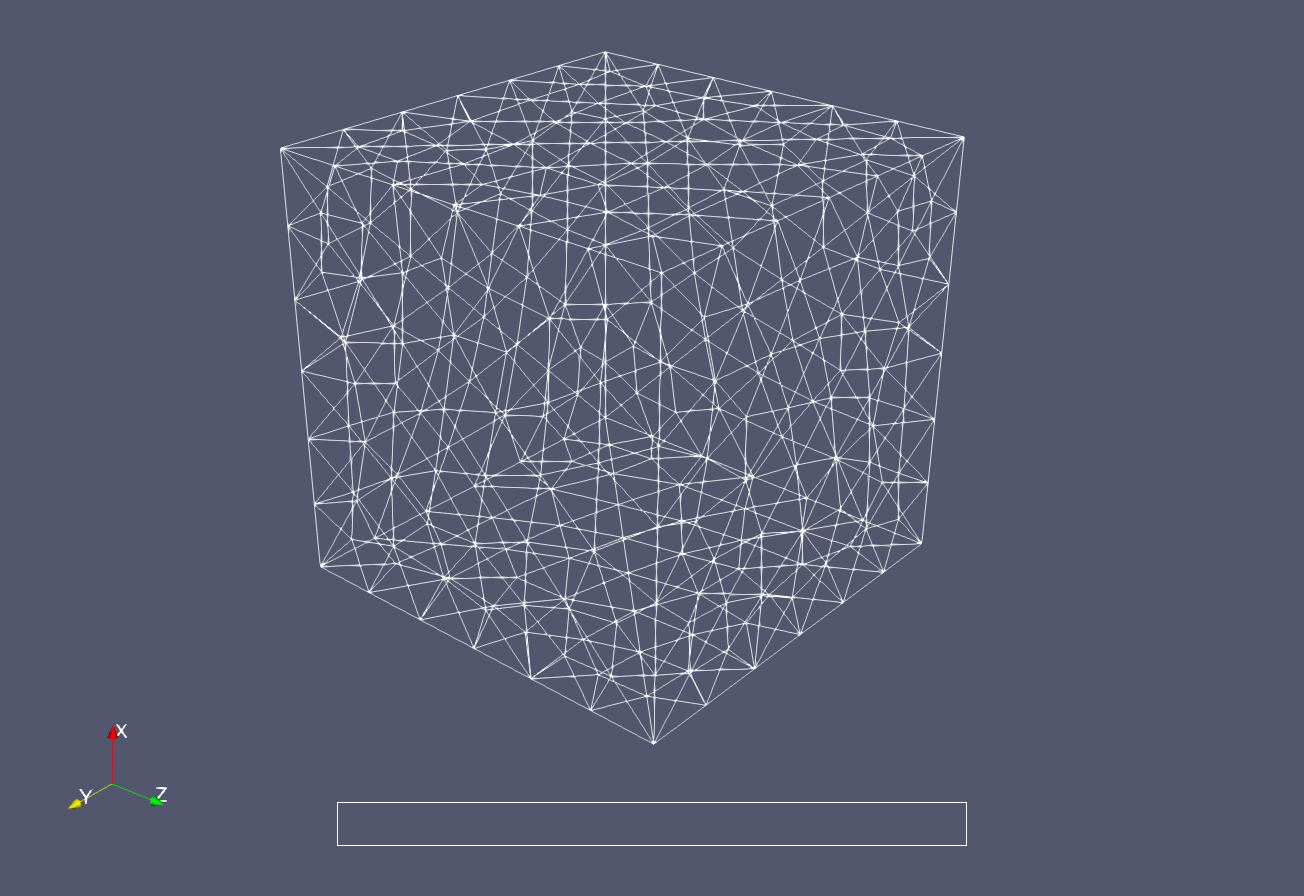
\includegraphics{img/mesh_0.2.png}
        \caption{The spatial mesh corresponding to \( \texttt{Mesh.MeshSizeMax} = 0.2 \), with 367 nodes and 1196 tetrahedral elements.}
        \label{fig:mesh-0.2}
    \end{subfigure}
    
    \begin{subfigure}{0.8\textwidth}
        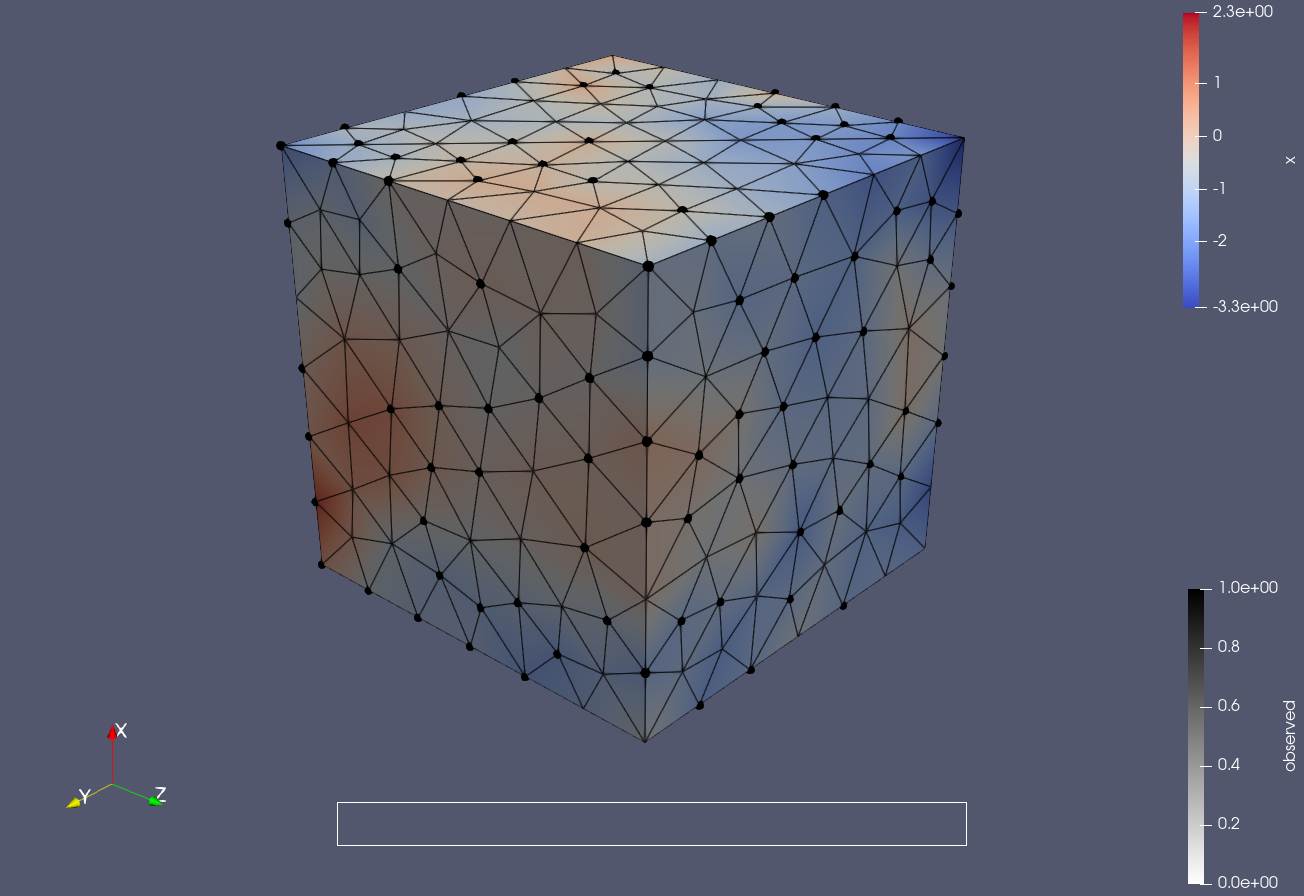
\includegraphics{img/mesh_0.2_x.png}
        \caption{A generated dataset for time-step \( t = 0 \).}
        \label{fig:mesh-0.2-x}
    \end{subfigure}
    \caption{Visualisation of the generated dataset \( \symbf{y} \).}
    \label{fig:mesh}
\end{figure}%
For the time domain, we choose a uniform discretisation with \( n_{t} \coloneqq 5 \) time-steps of length \( \increment t = 0.2 \). \Cref{eq:Q-st} becomes
\begin{equation}
    \symbf{Q}_{st} \approx \symbf{\tilde{Q}}_{st} = \gamma_{e}^{2} \left(
                           \symbf{Q}_{t, 1, 0}           \otimes \symbf{\tilde{Q}}_{s, 3, \gamma_{s}}
        + 2 \gamma_{t}     \symbf{Q}_{t, 1, \frac{1}{2}} \otimes \symbf{\tilde{Q}}_{s, 2, \gamma_{s}}
        +   \gamma_{t}^{2} \symbf{Q}_{t, 1, 1}           \otimes \symbf{\tilde{Q}}_{s, 1, \gamma_{s}}
    \right)
    \label{eq:Q-tilde}
    \text{,}
\end{equation}
as we are using the \gls{demf}(1, 2, 1) model (cf.\ \cref{sec:spatio-temporal-modelling}). We plot the sparsity pattern of \( \symbf{\tilde{Q}}_{st}\) in \cref{fig:Q-sparsity}.
\begin{figure}
    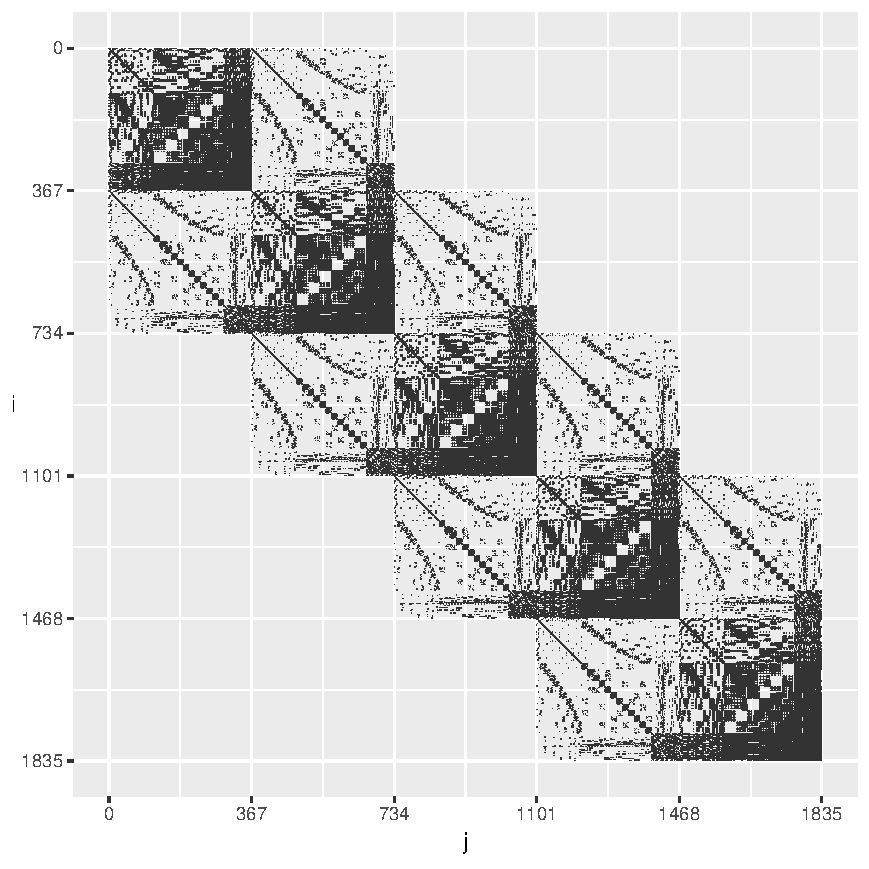
\includegraphics{img/Q_sparsity.pdf}
    % Q %>%
    %   as("TsparseMatrix") %>% 
    %   {tibble(x = .@j, y = .@i)} %>%
    %   ggplot(aes(x = x, y = y)) +
    %   geom_tile() +
    %   scale_x_continuous(name = "j", breaks = seq(from = 0, by = spatial_mesh$n, length.out = temporal_mesh$n + 1)) +
    %   scale_y_reverse(name = "i", breaks = seq(from = 0, by = spatial_mesh$n, length.out = temporal_mesh$n + 1)) +
    %   coord_fixed() +
    %   theme(axis.title.y = element_text(angle = 0, vjust = 0.5, hjust=1))
    \caption{The sparsity pattern of \( \symbf{\tilde{Q}}_{st} = (\tilde{q}_{i, j}) \). Recall that we have 367 spatial nodes and 5 time-steps in our mesh. The spatial mesh is clearly visible as blocks on the diagonal, replicated once for each time-steps. Due to the non-separable nature of the model, neighbouring time-steps are interconnected (compare \cref{eq:Q-tilde,eq:Qst-separable}).}
    \label{fig:Q-sparsity}
\end{figure}
Having the precision matrix allow us to sample from \( \symcal{N}(0, \symbf{\tilde{Q}}_{st}) + \symcal{N}(0, \sigma_{n}^{2}) \) to generate our noisy sample data \( \symbf{y} \). Note that the zero mean property of the field \( \symbf{u}(\symbf{x}, t) \) and the noise \( \symcal{N}(0, \sigma_{n}^{2}) \) can trivially guaranteed by centering the samples.

\section{Model fitting and parameter recovery}
\label{sec:fitting}
We split the generated dataset into two disjoint sets: a training dataset \( \symbf{y}_{\text{train}} \) consisting of \( \beta \) percent of the generated data, and a testing dataset \( \symbf{y}_{\text{test}} \) with the rest of the data. While we choose to perform the split only in space and not in time (i.e.\ data for a spatial point is either available for all time-steps, or for none of them)\textemdash{}in fact, not only can the availability of data vary both throughout space and time, but the observations need not even coincide with the mesh nodes, as they are interpolated unto them using the projector matrix \( \symbf{A} \in \symbb{R}^{N_{\text{data}} \times N_{\text{mesh}}} \). It can be constructed by transforming the global Cartesian coordinates of each data point into local coordinates of the element in which that data point resides\textemdash{}linearly interpolating in the time dimension and using barycentric coordinates for the spatial dimension. Since in our experiments data points always coincide with the mesh nodes, \( \symbf{A} \) takes the form of a unit matrix, with rows corresponding to unobserved points removed. Lastly, we specify priors on the model parameters \( \rho_{t} \), \( \rho_{s} \), \( \sigma_{e} \) and \( \sigma_{n} \), using penalised complexity priors~\cite{FuglstadConstructingpriorsthat2019}, where the parameter value used to synthesise the data is the median of the prior. We then invert the generating procedure, and attempt to fit a \gls{demf}(1, 2, 1) model to the training dataset \( \symbf{y}_{\text{train}} \).

Having fitted the model to the synthetic data, we compare the estimated parameters \( \rho_{t} \), \( \rho_{s} \), \( \sigma_{e} \) and \( \sigma_{n} \) to the values we used for model generation\textemdash{}and consider them successfully recovered if the generative value lies in the 95\% confidence interval (2.5\%\textendash{}97.5\%)\footnote{Note that the underlying processes are stochastic, and it cannot be expected that we always recover the generating value\textemdash{}the sample from \( \symbf{\tilde{Q}}_{st} \) might be extreme an have parameter values that are different from those we use to generate \( \symbf{\tilde{Q}}_{st} \)}; following the procedure outlined in the \texttt{inlamesh3d}~\cite{Lindgreninlamesh3d2022} vignette. Lastly, we visually inspect the model output by visualising it; which can be seen in \cref{fig:inla-results}.
\begin{figure}
    \centering
    \begin{subfigure}{0.8\textwidth}
        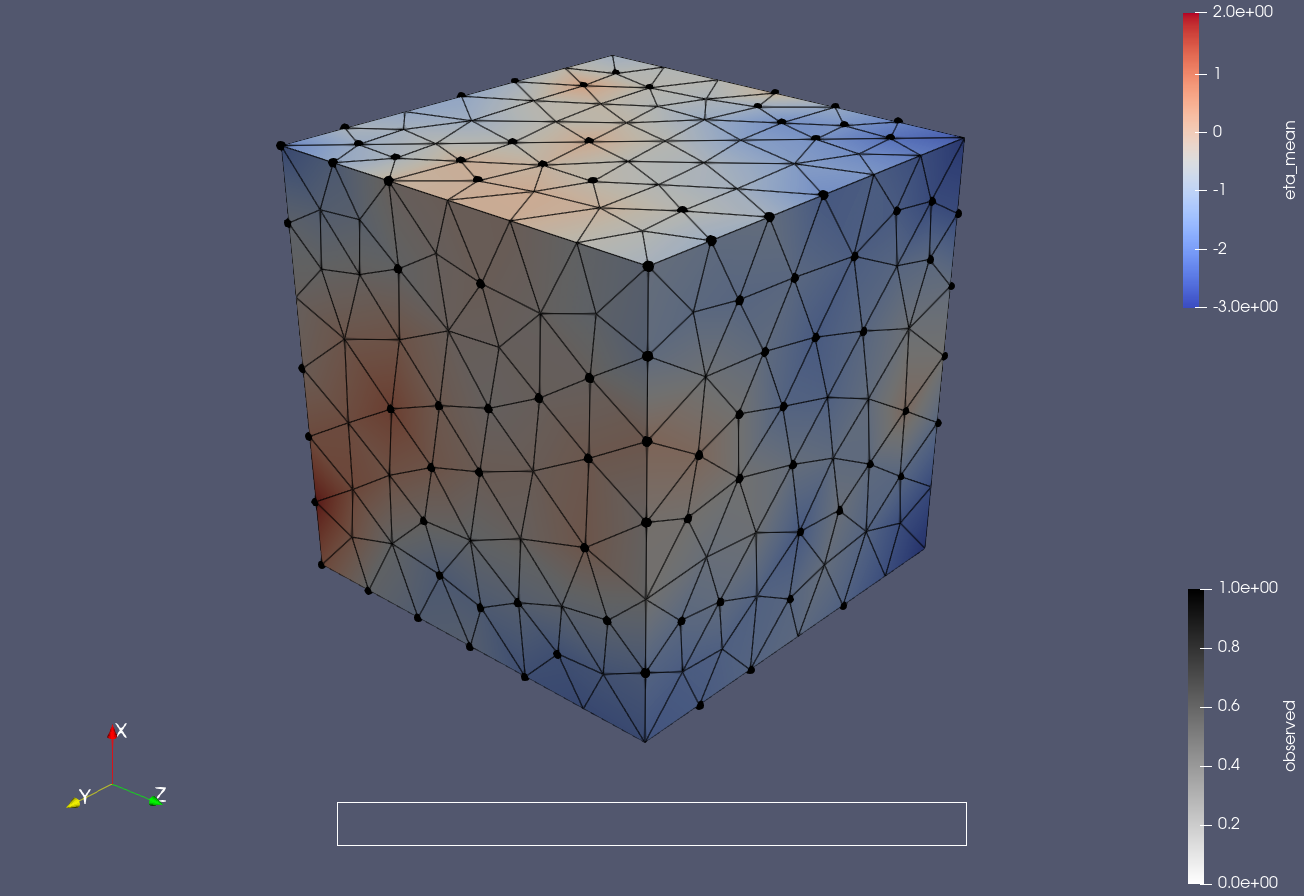
\includegraphics{img/mesh_0.2_eta.png}
        \caption{Mean of the posterior distribution, as predicted by \gls{inla}. Visual comparison with \cref{fig:mesh-0.2-x} shows little difference, which we interpret as good performance of the model.}
        \label{fig:mesh-0.2-eta}
    \end{subfigure}
    
    \begin{subfigure}{0.8\textwidth}
        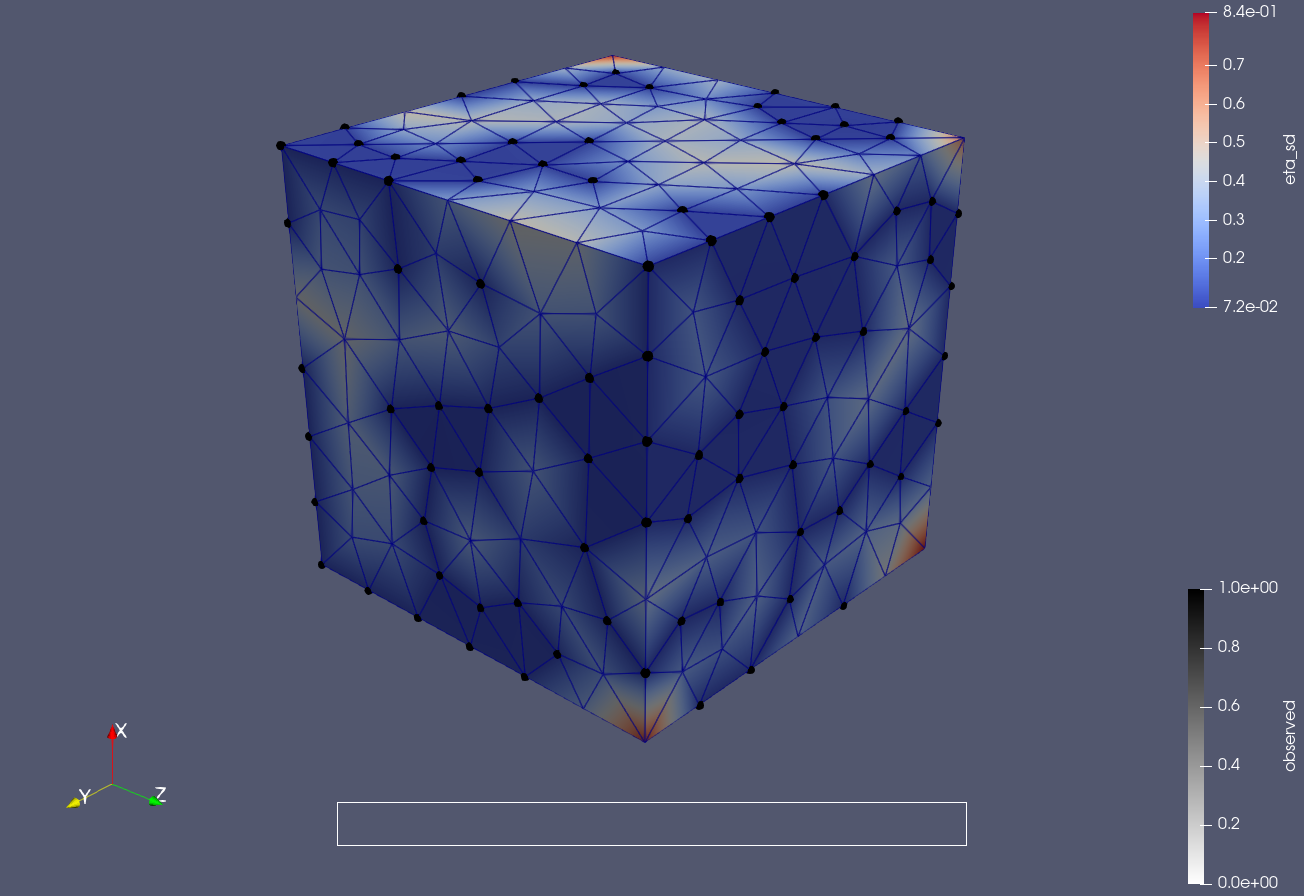
\includegraphics{img/mesh_0.2_sd.png}
        \caption{Plotted in colour is the standard deviation of the data, which can be taken as a measure of uncertainty of the model. Note, that it is smallest, where training data are present (denoted by black spheres), and increases, as the distance to these observations increases. Additionally, note that the uncertainty is the largest on the corner nodes, where no data is available, even when surrounded by other observations. This is a boundary effect, which would require adding ghost boundary cells to remediate.}
        \label{fig:mesh-0.2-sd}
    \end{subfigure}

    \caption{Visualisation the model, fitted to our synthetic data, using the same mesh as in \cref{fig:mesh-0.2}, at time-step \( t = 0 \).}
    \label{fig:inla-results}
\end{figure}

\chapter{Software and Code}
\label{ch:code}
Throughout the course of this work, multiple new R packages were developed~\cite{Sudwojinla3dt2022}: \texttt{tetgenr} and \texttt{gmshr} allow for interfacing with \texttt{TetGen}~\cite{SiTetGenDelaunayBasedQuality2015} and \texttt{Gmsh}~\cite{GeuzaineGmsh3Dfinite2009}; \texttt{meshr} provides a unified interface to different meshers, and outputs data in \gls{xdmf}~\cite{XDMF}; \texttt{inla3dt} provides functionalities needed for 3D + time modelling in \gls{inla}, which are not present in \texttt{INLA}, \texttt{inlamesh3d} or \texttt{INLAspacetime}. The above packages are detailed in the following sections. In \cref{sec:code-snippets}, we provide some useful code snippets, which might be of use to those wishing to replicate or build upon our work\textemdash{}these were either deemed to small as to warrant packaging, or were not generalisable enough to make into their own functions.

Additionally, we were able to make some contributions to the package \texttt{INLAspacetime}~\cite{KrainskiINLAspacetime2022}. These consist of commits
\texttt{\href{https://github.com/eliaskrainski/INLAspacetime/commit/1335173cf7b09b5030906a30797a1aeb9bf2ce9d}{1335173}},
\texttt{\href{https://github.com/eliaskrainski/INLAspacetime/commit/c598c492c1f19b18d72a427a3792cdaf047dae9c}{c598c49}},
\texttt{\href{https://github.com/eliaskrainski/INLAspacetime/commit/4b07d3782da6e109ab091a68fef07daffba3053c}{4b07d37}} and 
\texttt{\href{https://github.com/eliaskrainski/INLAspacetime/commit/6e3c9242ce432b2d636925950c917f6cb7ed93c5}{6e3c924}},
which make the package installable from source from within R, and, more importantly, add support for 3D + time models to that package.

\section{\texorpdfstring{\texttt{tetgenr}}{tetgenr}}
\label{sec:tetgenr}
The R package \texttt{tetgenr} is a thin wrapper around the \texttt{TetGen}~\cite{SiTetGenDelaunayBasedQuality2015} C \gls{api}. The newest version of the \texttt{TetGen} source code is bundled with the package, and gets built together with it. \texttt{tetgenr} exports one function, \mintinline{R}{tetgenr::mesh(...)}, which calls \texttt{TetGen}, and takes an \( (N \times 3) \) matrix of \( N \) point coordinates as the first argument, \texttt{geometry}, which should be meshed. A \( (M \times 3) \) matrix of boundary facets can be optionally provided in the second argument, \texttt{hull}, where each row are three \( 1 \)-based indexes into \texttt{geometry}, which form a boundary triangle facet. The order of the indexes does not matter, as the orientation of the facets will be corrected by the function. If \texttt{hull} is not supplied, will default to calculating the convex hull using Qhull~\cite{Barberquickhullalgorithmconvex1996} by calling \mintinline{R}{geometry::convhulln(...)}, if available; otherwise, an error will be thrown. Further arguments customisation of the meshing process, and map directly to \texttt{TetGen} options. The resulting mesh is returned as a named list, with \mintinline{R}{$geometry} being an \( (N' \times 3) \) matrix of point coordinates (depending on the options, points from the input may be inserted, deleted, or merged, to make the mesh adhere to the desired quality); and \mintinline{R}{$topology} a \( (M' \times 4) \) matrix of \( 1 \)-based point indices of the tetrahedral cells, which constitute the mesh. An example of usage can be seen in \cref{lst:tetgenr}.
\begin{listing}
    \begin{minted}{R}
        # define a unit cube
        spatial_domain <- rbind(
            c(0, 0, 0),
            c(0, 0, 1),
            c(0, 1, 0),
            c(0, 1, 1),
            c(1, 0, 0),
            c(1, 0, 1),
            c(1, 1, 0),
            c(1, 1, 1)
        )
        # mesh it
        spatial_mesh <- tetgenr::mesh(spatial_domain)
    \end{minted}
    \caption{Example use of \mintinline{R}{tetgenr::mesh}.}
    \label{lst:tetgenr}
\end{listing}
For further details, consult the package documentation~\cite{Sudwojinla3dt2022}.

\section{\texorpdfstring{\texttt{gmshr}}{gmshr}}
\label{sec:gmshr}
Similarly to \texttt{tetgenr}, the R package \texttt{gmshr} provides an R wrapper around the C++ \gls{api} of \texttt{Gmsh}~\cite{GeuzaineGmsh3Dfinite2009}, which is compiled with the package, and does not need to be installed on the system. The function \mintinline{R}{gmshr::mesh(...)} is called just like \mintinline{R}{tetgenr::mesh(...)}, and returns the same list structure. The difference lies in the extra optional arguments\textemdash{}here, any option that is understood by \texttt{Gmsh} is understood and can be set\textemdash{}see section \href{https://gmsh.info/doc/texinfo/gmsh.html#Gmsh-options}{\enquote{7\ Gmsh options}}, and, in particular, \href{https://gmsh.info/doc/texinfo/gmsh.html#Mesh-options}{\enquote{7.4 Mesh options}}, of the \href{https://gmsh.info/doc/texinfo/gmsh.html}{\texttt{Gmsh} manual}. An example call can be seen in \cref{lst:gmshr}, and further documentation is available with the package~\cite{Sudwojinla3dt2022}.
\begin{listing}
    \begin{minted}{R}
        spatial_mesh <- gmshr::mesh(
            spatial_domain,
            Mesh.MeshSizeMax       = 0.15,
            Mesh.OptimizeThreshold = 0.3,
            Mesh.QualityType       = 2,
            Mesh.OptimizeNetgen    = 1,
            Mesh.RecombineAll      = 1,
            Mesh.Recombine3DAll    = 1
        )
    \end{minted}
    \caption{Example usage of \mintinline{R}{gmshr::mesh(...)}, with some common meshing options set. \mintinline{R}{spatial_domain} is assumed to be the same as in \cref{lst:tetgenr}.}
    \label{lst:gmshr}
\end{listing}

\section{\texorpdfstring{\texttt{meshr}}{meshr}}
\label{sec:meshr}
The function of the R package \texttt{meshr} is two-fold: first, it provides a unified interface to the mesh-generating facilities of \texttt{geometry}, \texttt{tetgenr} and \texttt{gmshr}. Herewith, all three backends can be called with the same base arguments (\texttt{geometry} and optionally, \texttt{hull}) and return results in the same format (namely a list with members \mintinline{R}{$geometry} and \mintinline{R}{$topology}, as described in \cref{sec:tetgenr}). This allows for simple changing of the meshing backend, as can be seen in \cref{lst:meshr}.
\begin{listing}
    \begin{minted}{R}
        spatial_domain <- rbind(
            c(0, 0, 0),
            c(0, 0, 1),
            c(0, 1, 0),
            c(1, 0, 0)
        )
        spatial_hull <- matrix(1L:4L, nrow = 1, ncol = 4)
        # Mesh the same domain with three different backends
        spatial_mesh_qhull <- meshr::qhull(spatial_domain, spatial_hull)
        spatial_mesh_tetgen <- meshr::tetgen(spatial_domain, spatial_hull)
        spatial_mesh_gmsh <- meshr::gmsh(spatial_domain, spatial_hull)
        # convert any of them to INLA format
        spatial_mesh <- inlamesh3d::inla.mesh3d(
            loc = spatial_mesh_gmsh$geometry,
            tv  = spatial_mesh_gmsh$topology
        )
    \end{minted}
    \caption{The package \texttt{meshr} allows for easy exchange of meshing backends. Once a mesh has been generated, it can easily be translated into an \gls{inla}-compatible datastructure.}
    \label{lst:meshr}
\end{listing}

Second, \texttt{meshr} provides the function \mintinline{R}{meshr::write_xdmf(...)} to output a mesh to \gls{xdmf}~\cite{XDMF} format, for visualisation in external software such as ParaView~\cite{ParaView}. Both 2D and 3D meshes are supported; scalar and vector-valued attributes of nodes and cells can be specified through the arguments \texttt{node\_attributes} and \texttt{cell\_attributes}, respectively. These can also vary through time when passing a vector of time-steps via the argument \texttt{times}. Mesh geometry and topology is currently assumed to stay constant throughout time; this is only a limitation of the current implementation, and support could easily be implemented, if the need should arise.
\begin{listing}
    \begin{minted}{R}
        mesh <- list(
            geometry = rbind(
                c(0, 0, 0),
                c(0, 0, 1),
                c(0, 1, 0),
                c(1, 0, 0)
            ),
            topology = matrix(1L:4L, nrow = 1, ncol = 4)
        )
        meshr::write_xdmf(
            "mesh.h5",
            "mesh.xdmf",
            geometry = mesh$geometry,
            topology = mesh$topology,
            node_attributes = list(
                node_scalar = c(1, 2, 3, 4)
                node_vector = rbind(
                    c(1, 0, 0),
                    c(2, 0, 0),
                    c(3, 0, 0),
                    c(4, 0, 0)
                )
            ),
            cell_attributes = list(
                cell_scalar = c(-1),
                cell_vector = rbind(
                    c(-1, 0, 0)
                )
            )
        )
    \end{minted}
    \caption{Example of outputting of a \gls{xdmf} file, in three spatial dimensions, without time. \mintinline{R}{"mesh.h5"} and \mintinline{R}{"mesh.xdmf"} are the names of the files generated\textemdash{}the former is a \gls{hdf5}~\cite{HDF5LibraryFile} file containing the data, the latter a \gls{xdmf}~\cite{XDMF} file describing the former. The names of the elements of \texttt{node\_attributes} and \texttt{cell\_attributes} specify what the attribute will be called in ParaView~\cite{ParaView}. Values must be specified for each node or element; therefore, scalar attributes must have length \( N \), and vector-valued attributes must be \( (N \times d) \) matrices, where \( N \) is the number of nodes or elements, and \( d \) is the number of spatial dimensions (this is a limitation of the visualisation software, which can only display vectors of the same dimension as the mesh).}
    \label{lst:write-xdmf}
\end{listing}
\begin{listing}
    \begin{minted}{R}
        meshr::write_xdmf(
            "mesh.h5",
            "mesh.xdmf",
            geometry = mesh$geometry,
            topology = mesh$topology,
            times = c(0, 1),
            node_attributes = list(
                node_scalar = cbind(
                    c(1, 2, 3, 4),
                    c(5, 6, 7, 8)
                )
                node_vector = array(1:24, c(4, 3, 2))
            ),
            cell_attributes = list(
                cell_scalar = cbind(c(-1), c(-2))
                cell_vector = array(-1:-6, c(1, 3, 2))
            )
        )
    \end{minted}
    \caption{Example analogous to \cref{lst:write-xdmf}, with two time-steps, \( t = 0 \) and \( t = 1 \). Attribute values must be specified for all \( n_{t} \) time-steps, and therefore have dimensions \( (N \times n_{t}) \) and \( (N \times d \times n_{t}) \), when scalar-valued or vector-valued, respectively.}
    \label{lst:write-xdmf-time}
\end{listing}
Further documentation can be found alongside the package~\cite{Sudwojinla3dt2022}.

\section{\texorpdfstring{\texttt{inla3dt}}{inla3dt}}
\label{sec:inla3dt}
The package \texttt{inla3dt}~\cite{Sudwojinla3dt2022} implements functionality needed for defining 3D + time models in \gls{inla}. The function \mintinline{R}{inla3dt::mesh2fem(...)} generalises the functions \mintinline{R}{INLA::inla.mesh.2d.fem(...)}, \mintinline{R}{INLA::inla.mesh.fem(...)} and \mintinline{R}{inalmesh3d::inla.mesh3d.fem(...)}; calling the correct one and extending support to arbitrary \texttt{order}s. For 1D meshes, matrices \( \symbf{M}_{0} \coloneqq \symbf{Q}_{t, 1, 0} \), \( \symbf{M}_{1} \coloneqq \symbf{Q}_{t, 1, \sfrac{1}{2}} \) and \( \symbf{M}_{2} \coloneqq \symbf{Q}_{t, 1, 1} \) are additionally returned as \mintinline{R}{$m0}, \mintinline{R}{$m1} and \mintinline{R}{$m2}, respectively (cf.\ \cref{eq:C-t,eq:Q-t1,eq:Q-t2}).

The function \mintinline{R}{inla3dt::make_model_121(...)} defines a \gls{demf}(1, 2, 1) model. Depending on the argument \texttt{mode}, this is either the \texttt{cgeneric} model from the package \texttt{INLAspacetime} (\mintinline{R}{INLAspacetime::stModel.define(...)}) or the \texttt{rgeneric} model from this package\footnote{This was done when debugging the two versions\textemdash{}the \texttt{cgeneric} version is written in C, while the \texttt{rgeneric} version is written in R. Unsirprisingly, the \texttt{cgeneric} version is much faster}. The corresponding precision matrix \( \symbf{\tilde{Q}}_{st} \) can be generated using \mintinline{R}{inla3dt::make_Q(...)}\footnote{Note, that while it is possible to retrieve the precision matrix \( \symbf{\tilde{Q}}_{st} \) from the \texttt{rgeneric} model using \mintinline{R}{INLA::inla.rgeneric.q(...)}, the function \mintinline{R}{INLA::inla.cgeneric.q(...)$Q} does not accept passing \textit{\gls{spde} parameters} as arguments, returning a precision matrix for (arbitrary) default parameters instead.}, as demonstrated in \cref{lst:make-Q}. The function \mintinline{R}{inla3dt::interpretable2spde(...)} converts the \textit{interpretable model parameters} \( (\sigma_{e}, \rho_{s}, \rho_{t}) \) into the \textit{\gls{spde} parameters} \( \symbf{\gamma} = (\gamma_{t}, \gamma_{s}, \gamma_{e}) \) and the logarithm thereof, \( \symbf{\theta} = (\theta_{t}, \theta_{s}, \theta_{t}) \coloneqq (\ln(\gamma_{t}), \ln(\gamma_{s}), \ln(\gamma_{e})) \) as \mintinline{R}{$gamma} and \mintinline{R}{$theta} respectively; whereas the inverse is performed by \mintinline{R}{inla3dt::spde2interpretable(...)} (cf.\ \cref{eq:sigma-e,eq:rho-s,eq:rho-t}). Both of these transformations are implemented for arbitrary \gls{demf} models, and not only the \gls{demf}(1, 2, 1). To avoid bugs and confusion, we recommend passing arguments by name, and accessing the elements of \mintinline{R}{$gamma} and \mintinline{R}{$theta} by name as well (e.g.\ \mintinline{R}{$gamma[["s"]]} for \( \gamma_{s} \)).
\begin{listing}
    \begin{minted}{R}
        spatial_fem <- inla3dt::mesh2fem(spatial_mesh, order = 3L)
        temporal_fem <- inla3dt::mesh2fem(temporal_mesh)
        gamma <- inla3dt::interpretable2spde(
            sigma_e, rho_s, rho_t, d = 3,
            alpha = c(t = 1, s = 2, e = 1)
        )$gamma
        Q <- inla3dt::make_Q(spatial_fem, temporal_fem, gamma)
    \end{minted}
    \caption{Example use of \mintinline{R}{inla3dt::make_Q(...)}. Here, \mintinline{R}{spatial_mesh} and \mintinline{R}{temporal_mesh} are \gls{inla}~\cite{RueApproximateBayesianinference2009} mesh objects.}
    \label{lst:make-Q}
\end{listing}
Further documentation can be found alongside the package~\cite{Sudwojinla3dt2022}.

\section{Miscellaneous code snippets}
\label{sec:code-snippets}
We present here two miscellaneous code snippets, which the reader might find useful, but which do not warrant their own section, and which did not make it into any function.

First, in \cref{lst:A}, we demonstrate how the projector matrix \( \symbf{A} \) can be constructed for spatio-temporal models.
\begin{listing}
    \begin{minted}{R}
        spatial_A <- inlamesh3d::inla.mesh3d.make.A(spatial_mesh, loc)
        A <- INLA::inla.spde.make.A(
                A.loc      = matrix(1, temporal_mesh$n) %x% spatial_A,
                group      = rep(temporal_mesh$loc, each = nrow(loc)),
                group.mesh = temporal_mesh
            ) %>%
            zapsmall() %>%
            drop0()
    \end{minted}
    \caption{Creating the projector matrix \( \symbf{A} \). Let \texttt{spatial\_mesh} and \texttt{temporal\_mesh} be \texttt{INLA} mesh objects, and \texttt{loc} a vector of node indices at which observations are available. After creating the matrix, there might be some very small, non-zero entries\textemdash{} these are almost certainly numerical artefacts of the projection. Therefore they are set to zero (\mintinline{R}{zapsmall(...)}), and then explicit zero entries are deleted from the matrix (\mintinline{R}{Matrix::drop0(...)}), to increase its sparsity. We use the pipe operator (\texttt{\%>\%}) from \texttt{magrittr}/\texttt{tidyverse} purely for convenience.}
    \label{lst:A}
\end{listing}
Next, in \cref{lst:eta}, we show how we can extract summary statistics for the linear predictor from the \gls{inla}~\cite{RueApproximateBayesianinference2009} output, and make them ready for export via \mintinline{R}{meshr::write_xdmf}.
\begin{listing}
    \begin{minted}{R}
        library(tidyverse)
        eta <- est$summary.linear.predictor %>%
            rownames_to_column("var") %>%
            as_tibble() %>%
            mutate(
                kind = case_when(
                    str_detect(var, "^APredictor\\.") ~ "A",
                    str_detect(var, "^Predictor\\.")  ~ "meshpoint"
                ) %>% as.factor(),
                index = var %>% str_remove("^\\w+\\.") %>% as.integer()
            ) %>%
            select(
                kind,
                index,
                mean,
                sd,
                q_0.025 = `0.025quant`,
                q_0.5   = `0.5quant`,
                q_0.975 = `0.975quant`,
                d_kl    = kld
            ) %>%
            filter(kind == "meshpoint") %>%
            arrange(index)
    \end{minted}
    \caption{Extracting summary statistics from the linear predictor. Here, \texttt{est} is the output from \mintinline{R}{INLA::inla(...)}. The columns of \texttt{eta} can then be extracted and cast into matrices of adequate size, e.g.\ \mintinline{R}{matrix(eta$mean, n_nodes, n_timesteps)}, and passed as node attributes to \mintinline{R}{meshr::write_xdmf(...)}}.
    \label{lst:eta}
\end{listing}
Finally, in \cref{lst:field}, we do the same for the summary statistics of the fitted field \( \symbf{u}(\symbf{x}, t) \),
\begin{listing}
    \begin{minted}{R}
        library(tidyverse)
        field <- est$summary.random$field %>%
        	as_tibble() %>%
        	select(
        		index = ID,
        		mean,
        		sd,
        		q_0.025 = `0.025quant`,
        		q_0.5   = `0.5quant`,
        		q_0.975 = `0.975quant`,
        		d_kl    = kld
        	) %>%
        	mutate(index = as.integer(index))
    \end{minted}
    \caption{Analogous example to \cref{lst:eta}, for preparing the field summary statistics for export and plotting.}
    \label{lst:field}
\end{listing}

\chapter{Conclusion}
\label{ch:conclusion}
In this thesis, we have shown how to fit 3D + time spatio-temporal models in \texttt{R-INLA}. We provide facilities for generating three-dimensional meshes in R, by providing interfaces to two well known meshers, \texttt{TetGen}~\cite{SiTetGenDelaunayBasedQuality2015} and \texttt{Gmsh}~\cite{GeuzaineGmsh3Dfinite2009}, and interactive visualisation in ParaView~\cite{ParaView}; facilities which we find crucial for working with 3D + time models. Our testing procedure, as outlined in \cref{sec:extending}, should prove valuable during the process of adding this functionality to official versions of \texttt{R-INLA}.

To conclude this work, we sketch what we envision might be a possible future for spatio-temporal modelling with \texttt{R-INLA}. First, we would welcome if functionalities from both \texttt{inlamesh3d}~\cite{Lindgreninlamesh3d2022} and \texttt{INLAspacetime}~\cite{KrainskiINLAspacetime2022} would be integrated into \texttt{R-INLA}, so that they are supported on par with other parts of the programme\textemdash{}to our knowledge, this is planned or already underway. Second, demonstration of more complex 3D + time models would be beneficial; as would the application to real-world datasets and problems\textemdash{}both of these would, in out opinion, show the viability of 3D + time modelling with \texttt{R-INLA}, and provide domain scientists with a stepping stone or foundation, upon which they can build their models. We consider MRI, meteorological and pollution data to be good first candidates for such a demonstration. It would also be interesting to compare the model performance of \gls{inla} to more physically informed models, e.g.\ how well can \gls{inla} model diffusion or heat transfer, compared to state-of-the-art numerical methods. Third, mesh generation could be improved, e.g.\ by adding support for ghost boundary cells in 3D to compensate for boundary effect artefacts. Since \gls{inla} is agnostic as to the underlying mesh topology, the use of meshes whose spatial structure changes through time could be explored, for example using the recently developed \texttt{avro} 4D-mesher~\cite{Caplanavro, CaplanFourdimensionalanisotropicmesh2020}. Finally, the impact of adding a third spatial dimension on performance is not clear, and might need further investigation.

\appendix
% \nocite{*}
\printbibliography[heading = bibnumbered]

\printglossaries

\chapter{Notation}
\label{ch:notation}
\begin{itemize}
    \item \( \symbf{x} \): vector
    \item \( \symbf{A} \): matrix
    \item \( \prob(x) \): probability of event \( x \)
    \item \( \mu \): mean
    \item \( \sigma \): standard deviation
    \item \( \sigma^{2} \): variance
    \item \( \cov(x, y) \): covariance of \( x \) and \( y \)
    \item \( \cor(x, y) \): correlation of \( x \) and \( y \)
    \item \( \symup{\Gamma}(z) \): Gamma function
    \item \( \BesselK_{\alpha}(z) \): modified Bessel function of the second kind of order \( \alpha \)
    \item \( \psi_{i} \): \gls{fem} basis function
    \item \( \phi_{i} \): \gls{fem} basis function
    \item \( \langle f, g \rangle \): inner product
    \item \( G \graphprod H \): \cref{def:graph-product}
    \item \( u \adj v \): \( u \) is adjacent to \( v \)
    \item \( K_{n} \): complete graph of order \( n \)
    % \item \( Q_{n} \): hypercube graph of dimension \( n \)
    % \item \( C_{n} \): cycle graph of girth \( n \)
\end{itemize}

\clearpage
\phantomsection
\stepcounter{chapter}
\addcontentsline{toc}{chapter}{\protect\numberline{\thechapter}{Declaration of originality}}
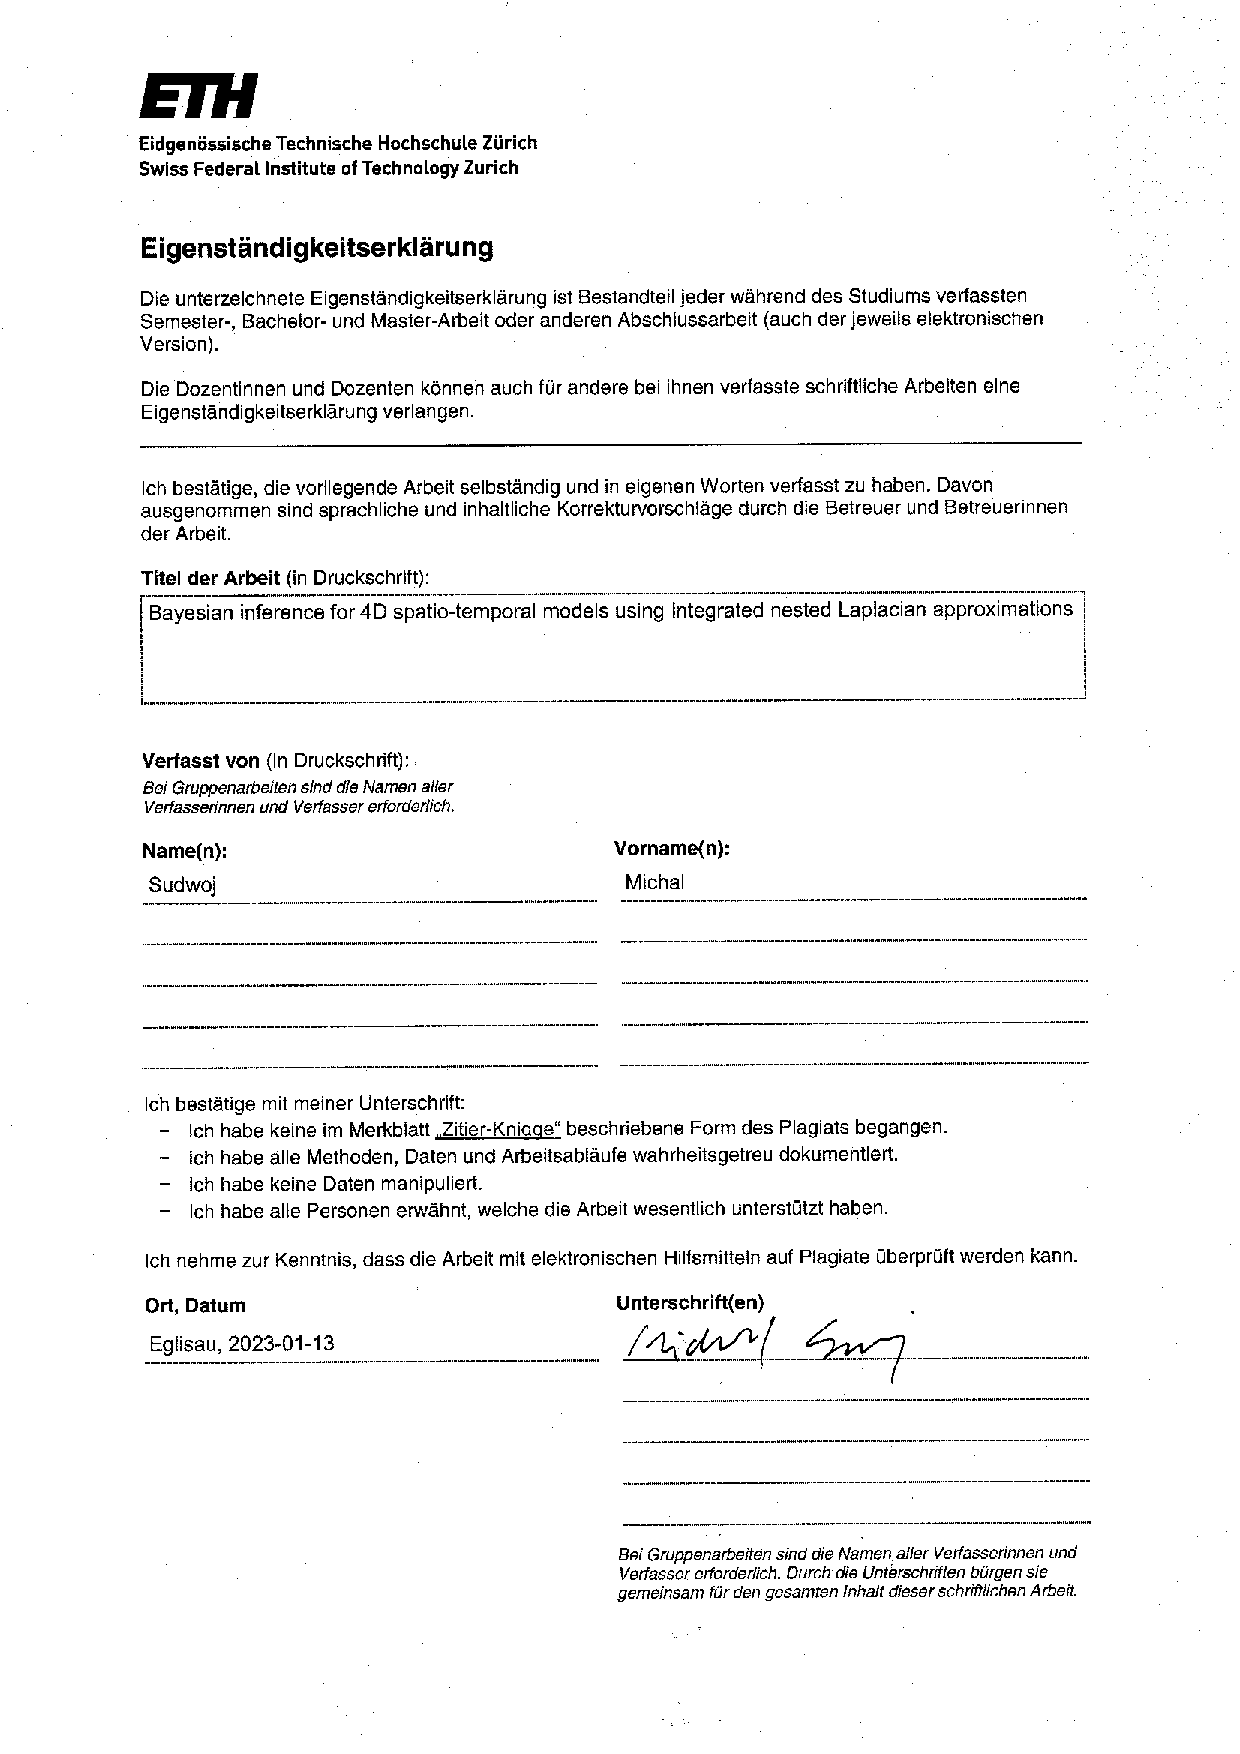
\includepdf[pages=-]{declaration-originality-signed}

\end{document}
\endinput